\documentclass[11pt, oneside]{book} % for compiling digital distributions
% \documentclass[11pt, twoside]{book} % for compiling for physical prints
% General packages
\usepackage[english]{babel}
\usepackage{hyperref}
\usepackage[utf8]{inputenc}

\usepackage[nottoc,notlot,notlof]{tocbibind}

% Set page layout
\usepackage[
  a4paper,
  includehead,       % Header is within page margins
  headheight=0.6cm,  % Always present (regardless of text)
  inner=2.5cm,
  outer=1.5cm,
  top=2cm,
  bottom=2cm
  ]{geometry}

% Suppress default required title
\renewcommand\maketitle{}

% To set line spacing to 1
\usepackage{setspace}
\singlespacing

% Some generally useful packages that you may or may not need
\usepackage[ruled,vlined]{algorithm2e}
\usepackage[toc, page]{appendix}
\usepackage[font=small,labelfont=bf]{caption}
\usepackage{fancyhdr}
\usepackage{float}
\usepackage[T1]{fontenc}
\usepackage{listings}
\usepackage{makecell}
\usepackage{multicol}
\usepackage{soul}
%\usepackage{textcomp} % commented due to clash
\usepackage{wrapfig}
\usepackage{xcolor}
\usepackage{graphicx}
\usepackage{lmodern}
\usepackage{tcolorbox}

% Math packages
\usepackage{amsfonts}
\usepackage{amsmath}
\usepackage{dsfont}
\usepackage{mathtools}

% Set font to Times New Roman
\usepackage{newtxtext}  % Times-like text font
\usepackage{newtxmath}  % Times-like math font

\usepackage{subcaption}

% Some general page settings from
% https://github.com/giacThePhantom/MolecularPhysics
\pagestyle{fancy}

%\renewcommand{\familydefault}{\sfdefault} %% this line prevents the conversion to Times New Roman, as it changes the default font family to serif

% avoid indentation and preserve new lines from Markdown
\setlength{\parindent}{0pt}
\setlength{\parskip}{6pt plus 2pt minus 1pt}

\fancyhf{}
\lhead{\rightmark}
\cfoot{\leftmark}
\rfoot{\thepage}

\setcounter{secnumdepth}{5}

\lstset{
    frame=tb, % draw a frame at the top and bottom of the code block
    tabsize=4, % tab space width
    showstringspaces=false, % don't mark spaces in strings
    numbers=none, % display line numbers on the left
    commentstyle=\color{green}, % comment color
    keywordstyle=\color{red}, % keyword color
    stringstyle=\color{blue}, % string color
    breaklines=true,
    postbreak=\mbox{\textcolor{green}{$\hookrightarrow$}\space}
}

\providecommand{\tightlist}{%
  \setlength{\itemsep}{0pt}\setlength{\parskip}{0pt}}


\begin{document} % full document should have min 26, max 85 pages, excluding reference list and any appendices
  \pagenumbering{gobble} % don't add page numbers
  \pagestyle{empty}
\begin{center}
  \begin{figure}[h!]
    \centerline{
\psfig{file = figures/logo_unitrento.eps, width=0.6\textwidth}}
  \end{figure}

  \vspace{1 cm}
  \Large{Master's Degree thesis in\\Quantitative and Computational Biology\\}
  \vspace{1 cm}

  \LARGE\textsc{Physical characterization of protein and rna binding sites and their graphical representation in the molecular visualization software UnityMol\\}
  \vspace{0.5 cm}
  \LARGE{Diego Barquero Morera\\}
  \vspace{0.5 cm}
  \Large{Supervisor: Samuela Pasquali\\}
  \Large{Co-supervisor: Luca Tubiana\\}

  \vspace{2 cm}
  \Large{Department of Cellular, Computational and Integrative Biology - CIBIO\\}
  \Large{Università degli studi di Trento}
  \vspace{0.5 cm}

  \Large{Academic year: 2023/2024}\\
  \Large{Discussion date: 14/12/2023}
\end{center}
\maketitle


  \tableofcontents

  \cleardoublepage \pagenumbering{arabic} % start page number on abstract
  %%% short summary, that provides the context and the objectives of the project, and summarizes the scientific problem, the techniques used and the results obtained
%%% In case of collaborative work, here is where the graduating student gives details on their contribution to the study
\chapter*{Abstract} % about 1 page in length
\addcontentsline{toc}{chapter}{Abstract}

The development of molecular visualization software plays an important role in many fields of molecular biology, such as the computer-aided drug discovery and design. Understanding the physical properties of binding pockets of target macromolecules, such as certain proteins and RNAs, is key in designing effective ligands for desired outcomes. Several interactions can occur between a binding pocket and its ligands, such as electrostatics, $\pi$-stacking, hydrogen bonds and hydrophobic effects, among others.

This prototype consisted of characterizing the physicochemical properties of the binding sites, developing visualization methods appropriate for the numerical results obtained, and benchmarking the whole pipeline with interesting protein and RNA systems. For the first step, mathematical models based in theoretical considerations and a statistical analysis (for the stacking interaction) were conceived. A visualization workflow was developed based in the framework provided by UnityMol, that allows users to define the volume of interest for a binding pocket, calculate their potentials and visualize the results. The volumetric data was mostly represented by isosurfaces, although a new visualization method was also proposed, denominated here \textit{cloud representation}.

The 10 protein and 10 RNA benchmarks provide multiple examples of how the prototype behaved under different circumstances. Results were varied, with the stacking potential having a great overall performance, followed by clear visualizations for the hydrophobic interactions. The electrostatic potential can still be polished in terms of visualization, while the hydrogen bonds potentials need to have their modelling and visualization aspects improved.

Altogether, the models and visualization workflow proposed in this prototype provide new insights into molecular systems of biological interest. It also serves as a proof of concept and a starting point for implementing further methodologies in a relatively unexplored molecular visualization niche, namely the physical characterization and representation of volumes of interest in molecular systems.

  %%% background to the research work
\chapter{Introduction} % at least 5 pages, not more than 10

%%%%%%%%%%%%%%%%%%%%%%%%%%%%%%%%%%%%%%%%%%%%%%%%%%%%%%%%%%%%%%%%%%%%%%%%%%%%%%%%
\section{Computer-aided Drug Discovery and Design}
  \subsection{Computational Methods}
    In the last decades, the development of new pharmaceuticals has been significantly boosted by the field of \textit{computer-aided drug discovery and design}. Computational methods allow to automate the exploration of a huge space of molecule configurations, with the goal of predicting which compounds would elicit desired biologic responses, and which others can be disregarded. According to these predictions, the molecules with the most therapeutic potential can be prioritized in further experimental stages, saving time and resources in the process of finding new benefitial drugs \cite{drug_discovery_2014}.

    Computational methods for drug discovery can be categorized in two main branches: \textit{ligand-based} (LBDD) and \textit{structure-based} (SBDD). Ligand-based methods focus only in the ligand and try to predict the behaviour of new molecules by taking as reference the activity of other known strucurally similar ligands. Structure based methods use information from the 3D structures of both ligand and target, and include approaches such as \textit{ligand docking}, \textit{molecular dynamics simulations} and \textit{pharmacophore modeling} \cite{drug_discovery_2014, structure_based_2019}.

  \subsection{Target Molecules and Binding Pockets}
    Although SBDD methods require the additional knowledge of the target structure (which is not trivial), they have been proven to be powerful and efficient methods in drug discovery \cite{structure_based_2019}. Consequently, the first basic step of SBDD methods is resolving the 3D structure of the therapeutically important \textbf{target molecule}, which traditionally refers to some protein of interest \cite{structure_based_2019}. However, this is not always the case, as in more recent years relevant RNA structures have also started to be considered as target molecules \cite{rna_targets_2022}.

    \begin{figure}[H]
      \centering
      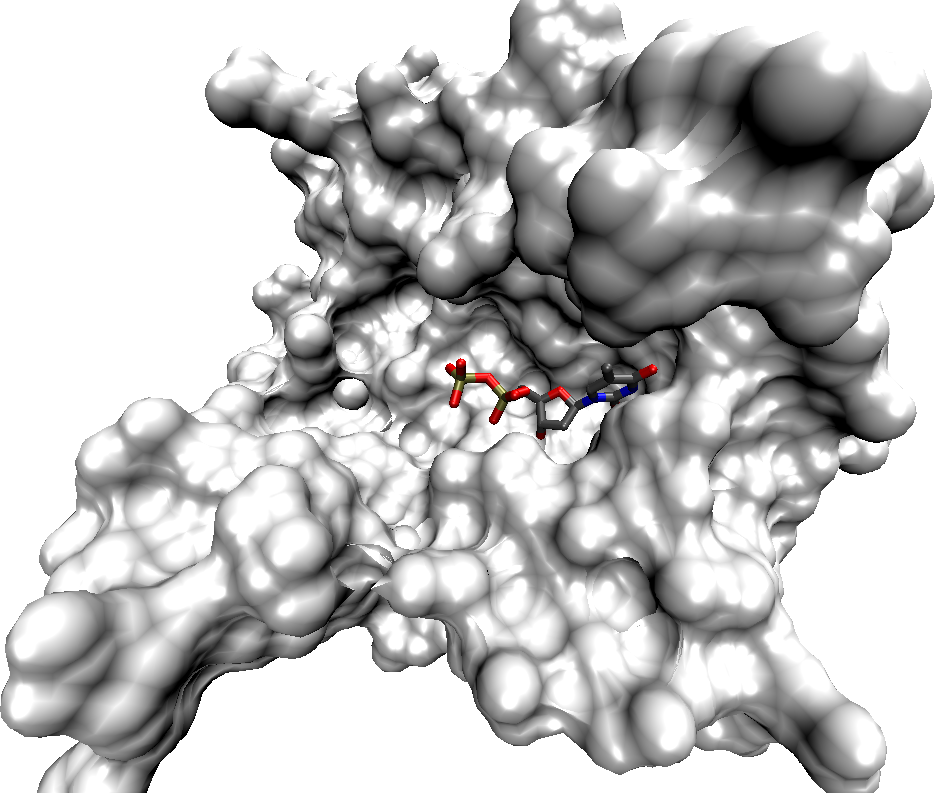
\includegraphics[width=0.5\textwidth]{figures/intro/pocket.png}
      \caption{\label{fig:intro/pocket} Ligand bound to the pocket of a protein (PDB: 1h7l).}
    \end{figure}

    Once the structure of the target is well known, an appropriate \textbf{binding pocket} must be identified. This refers to a small cavity in the target where a ligand should bind to produce the desired effect (figure \ref{fig:intro/pocket}). Once this binding site is identified, different SBDD techniques can be performed, such as \textit{virtual screening}, \textit{de novo drug design}, \textit{molecular docking} and \textit{pharmacophore modeling}, among others \cite{drug_discovery_2014, structure_based_2019, pharmacophore_and_VS_2022}.

  \subsection{Virtual Screening and Pharmacophores}
    \textbf{Virtual screening} is a series of computational methods where a dataset of chemical compounds is reduced to only those with some chemical characteristics of interest, which generally means those with higher binding affinity to a given target pocket \cite{pharmacophore_and_VS_2022, virtual_screening_2019}. Given the immense chemical space of potential ligands, with curated databases consisting of millions of compounds, blindly performing virtual screening over whole datasets is often unpractical \cite{virtual_screening_2013}. This process can be however optimized by using \textit{pharmacophores} to reduce the search space to only those molecules that best satisfy some desired properties \cite{pharmacophore_and_VS_2022}.

    \textbf{Pharmacophore} models describe the spatial arrangement of steric and electronic features that allow ligands to optimally interact with their target binding sites \cite{pharmacophore_and_VS_2022, virtual_screening_2019, pharmacophore_modeling_2022, drug_discovery_2014}. The core idea behind pharmacophores is that ligands with common physicochemical properties and spatial arrangements should have a similar biological activity on the same target. The most relevant pharmacophoric features include \textit{positively and negatively charged groups}, \textit{aromatic groups}, \textit{hydrogen bond acceptors/donors}, \textit{hydrophobic areas}, \textit{exclusion volumes}, among others (figure \ref{fig:intro/pharmacophores}) \cite{pharmacophore_and_VS_2022, drug_discovery_2014}.

    \begin{figure}[H]
      \centering
      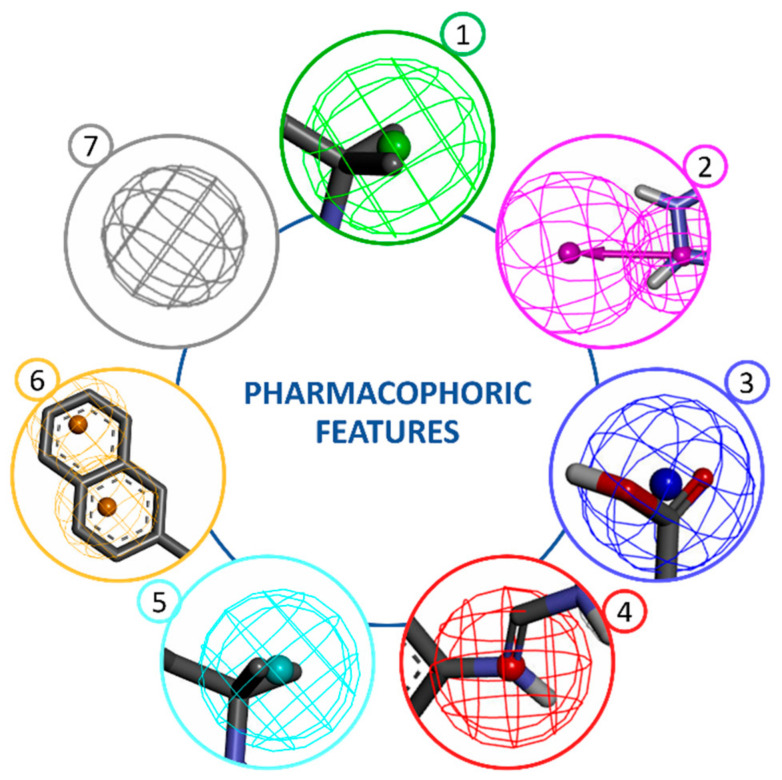
\includegraphics[width=0.5\textwidth]{figures/intro/pharmacophores.jpg}
      \caption{\label{fig:intro/pharmacophores} Summary of the main pharmacophoric features. 1) hydrogen bond acceptors, 2) hydrogen bond donors, 3) negatively charged, 4) positively charged, 5) hydrophobic, 6) aromatic, 7) exclusion volume. Adapted from \cite{pharmacophore_and_VS_2022}.}
    \end{figure}

    Pharmacophores can be modeled in either LBDD or SBDD pipelines. In the case of a structure-based approach, the pharmacophore can be obtained by different strategies. A completely target-based method can be employed, in which the pharmacophoric features are inferred by performing an analysis of the binding pocket's structure \cite{pharmacophore_and_VS_2022, virtual_screening_2019}.

    A more experimental approach involves molecular docking of different molecules from a ligand dataset, clustering the fragments with best affinity and extracting pharmacophore features from these clusters. Another straightforward and still effective strategy can be followed when experimental structures of target-ligand complexes are available. In this case, the pharmacophore features can be built based on this ligand, whose bioactive conformation is already known \cite{virtual_screening_2019}.


%%%%%%%%%%%%%%%%%%%%%%%%%%%%%%%%%%%%%%%%%%%%%%%%%%%%%%%%%%%%%%%%%%%%%%%%%%%%%%%%
\section{Physicochemical Properties of the Binding Sites}
  \subsection{Binding Affinity}
    From a chemical point of view, the interaction between ligand and target binding site can be considered as a \textit{binding reaction}, where the substrates are the ligand and the target, and the product is the target-ligand complex. The free energy of such reaction is therefore associated with how strongly the ligand binds to the target \cite{binding_affinity_2016, binding_affinity_web}.

    This concept, denominated \textbf{binding affinity}, is usually measured by the equilibrium dissociation constant $K_D$. At smaller $K_D$ values there is a greater binding affinity between ligand and target, while at larger $K_D$ values their interaction is weaker. As so, knowing which factors affect the binding affinity is key to designing optimal pocket-ligand interactions \cite{binding_affinity_web}.

    Binding affinity is mainly influenced by non-covalent intermolecular interactions between the target pocket and the ligand. This include \textit{ionic or electrostatic interactions}, \textit{stacking}, \textit{hydrogen bonds}, \textit{hydrophobic effects and van der Waals forces}, \textit{metal bonding}, \textit{desolvation}, among others \cite{binding_affinity_2016, binding_affinity_web, electrostatics_2020, stacking_binding_2020, stacking_trp_2022, hbonds_2023, hydrophobic_2017, hydrophobic_2022}.

    Computational methods behind binding affinity calculations often involve \textbf{energy functions}, which are based either on physical description of these interactions or on statistical analyses of experimentally characterized ligands. \textit{Physical energy functions} can contain terms common in molecular dynamics force fields, such as: bond stretching; angles bending, rotation and torsion; coulombic interactions; van der Waals attraction; exchange repulsion and others. On the other hand, \textit{statistical energy functions} often rely on distances between atoms to build an empirical potential of mean force, by taking into account the physicochemical properties that affect binding affinity \cite{binding_affinity_2016}.

  \subsection{Electrostatics}
    Binding affinity is greatly affected by the \textbf{electrostatic interactions} between positively and negatively charged groups in oposing molecules (figure \ref{fig:intro/electrostatics}). This contribution is even higher when intermolecular ion pairs (salt bridges) are formed. It is important to note that under physiological conditions, the presence of ions in the solvent further impact the electrostatic behaviour of the molecules. As RNA molecules are highly negatively charged, cations tend to condense near their surface. On the other hand, proteins tend to attract both anions and cations, but with less intensity. Either way, the long range nature of electrostatic forces and the abundance of charged amino and nucleic acids make this interactions particularly relevant \cite{electrostatics_2020, electrostatics_2019, apbs_2004}.

    \begin{figure}[H]
      \centering
      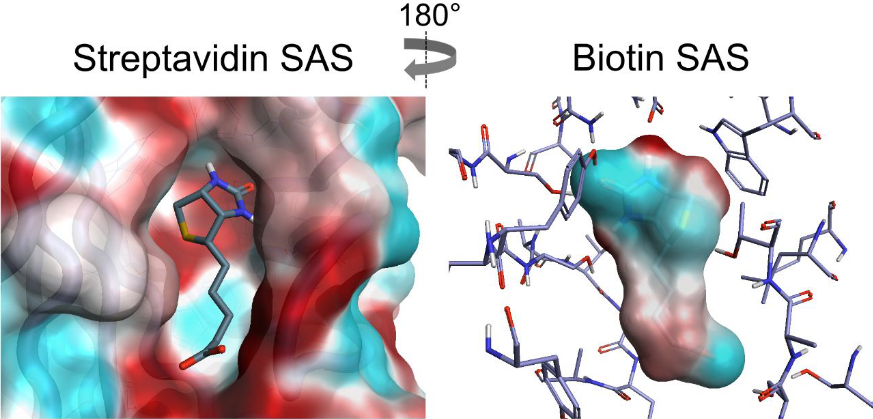
\includegraphics[width=0.5\textwidth]{figures/intro/electrostatics.png}
      \caption{\label{fig:intro/electrostatics} Electrostatic interaction between ligand (biotin) and target protein (streptavidin) forming a complex (PDB: 3RY2). Blue) negative electrostatic potential, Red) positive electrostatic potential. Adapted from \cite{electrostatics_2019}.}
    \end{figure}

    A standard method for studying biomolecular electrostatics consists of solving the Poisson-Boltzmann equation of continuum electrostatics, which incorporates information about the molecular shape and charge distribution. This is best solved numerically with a grid-based and finitely-discretized approach. The \textbf{Adaptive Poisson–Boltzmann Solver} (APBS) software provides a flexible and powerful pipeline for this purpose \cite{apbs_2004, apbs_2018, apbs_web}.

  \subsection{Stacking}
    The presence of $\pi$-stacking interactions can also contribute to a higher binding affinity in ligand binding. This kind of interaction is traditionally considered to happen between two \textit{aromatic groups}, which are notable for their planarity and $\pi$-electron cloud over and under the aromatic ring plane. Whenever their spatial placement allow for this clouds to interact in a particular way, a \textbf{stacking interaction} occurs. The chemical details behind this phenomenon are still not fully understood and is still object of debate, which also means their quantification and modeling is not straightforward \cite{stacking_binding_2020, stacking_trp_2022, stacking_general_2020}.

    \begin{figure}[H]
      \centering
      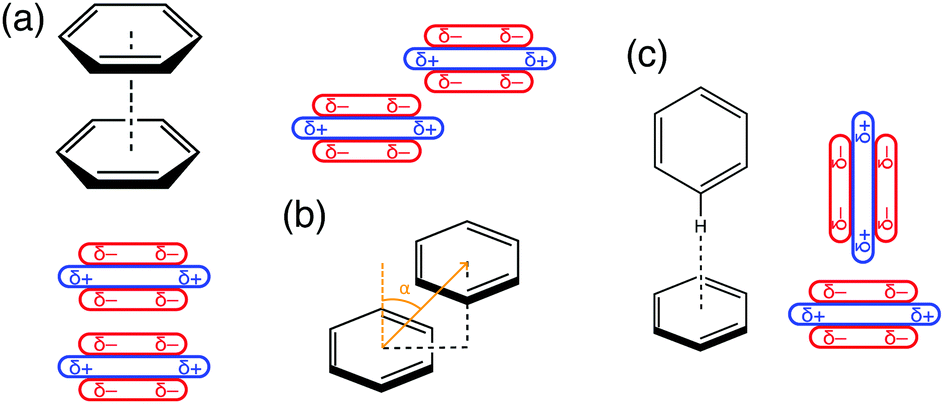
\includegraphics[width=0.5\textwidth]{figures/intro/stacking_configs.png}
      \caption{\label{fig:intro/stacking_configs} [TODO] description. Adapted from \cite{stacking_general_2020}.}
    \end{figure}

    The spatial configuration of the aromatic rings play a fundamental role in stacking interactions. This can be summarized by three spatial degrees of freedom: distance, $\alpha$ angle and $\beta$ angle. The $\alpha$ angle describes how tilted the center of geometry is from one ring with respect to the other ring, while $\beta$ is the angle between the vectors normal to the planes (figures \ref{fig:intro/stacking_configs} and \ref{fig:intro/stacking_angles}) \cite{stacking_general_2020, rna_2015}.

    \begin{figure}[H]
      \centering
      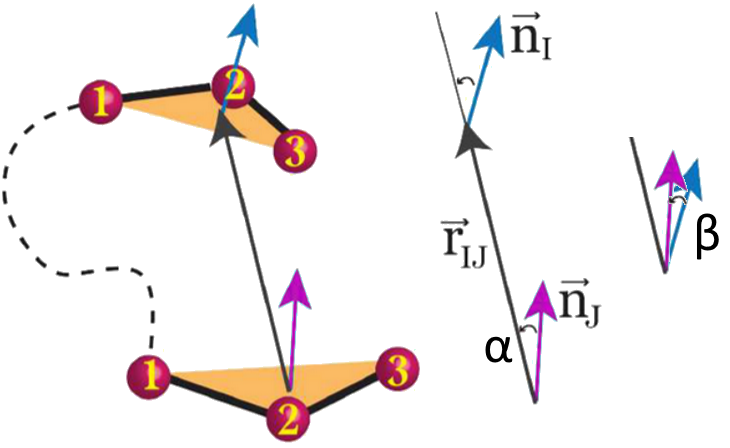
\includegraphics[width=0.5\textwidth]{figures/intro/stacking_angles.png}
      \caption{\label{fig:intro/stacking_angles} [TODO] description. Adapted from \cite{rna_2015}.}
    \end{figure}

    The traditional \textbf{$\pi$-$\pi$ stacking} is considered to be optimal when $\alpha>0$ (but still a low value) and $\beta \approx 0$, yielding a \textit{parallel-offset} geometry. The alternative \textbf{CH-$\pi$ stacking} also represents an energetic local minimum, with $\alpha \approx 0$ and $\beta \approx 90^{\circ}$, which corresponds to a \textit{perpendicular} geometry (figure \ref{fig:intro/stacking_configs}) \cite{stacking_general_2020}.

    It is also noteworthy that aromatic rings can also interact in other similar ways to $\pi$-$\pi$ and CH-$\pi$ stacking. These include \textit{cation-$\pi$}, \textit{amid-$\pi$}, \textit{amid-$\pi$} and \textit{halogen-$\pi$} \cite{stacking_binding_2020, electrostatics_2020}.

  \subsection{Hydrogen Bonds}
    Another kind of interaction fundamental for the structure of macromolecules and their binding affinity to ligands is the presence of \textbf{hydrogen bonds}. These are weak interactions that happen between so-called \textit{donor} and \textit{acceptor} atom pairs, under an appropriate distance and angle. A \textbf{donor} is an electronegative atom such as nitrogen (N), oxygen (O) or fluor (F) covalently bound to a hydrogen (H) atom, while an \textbf{acceptor} is an electronegative atom with a lone pair of electrons or a negative charge (figure \ref{fig:intro/hbonds}) \cite{hbonds_2023}.

    \begin{figure}[H]
      \centering
      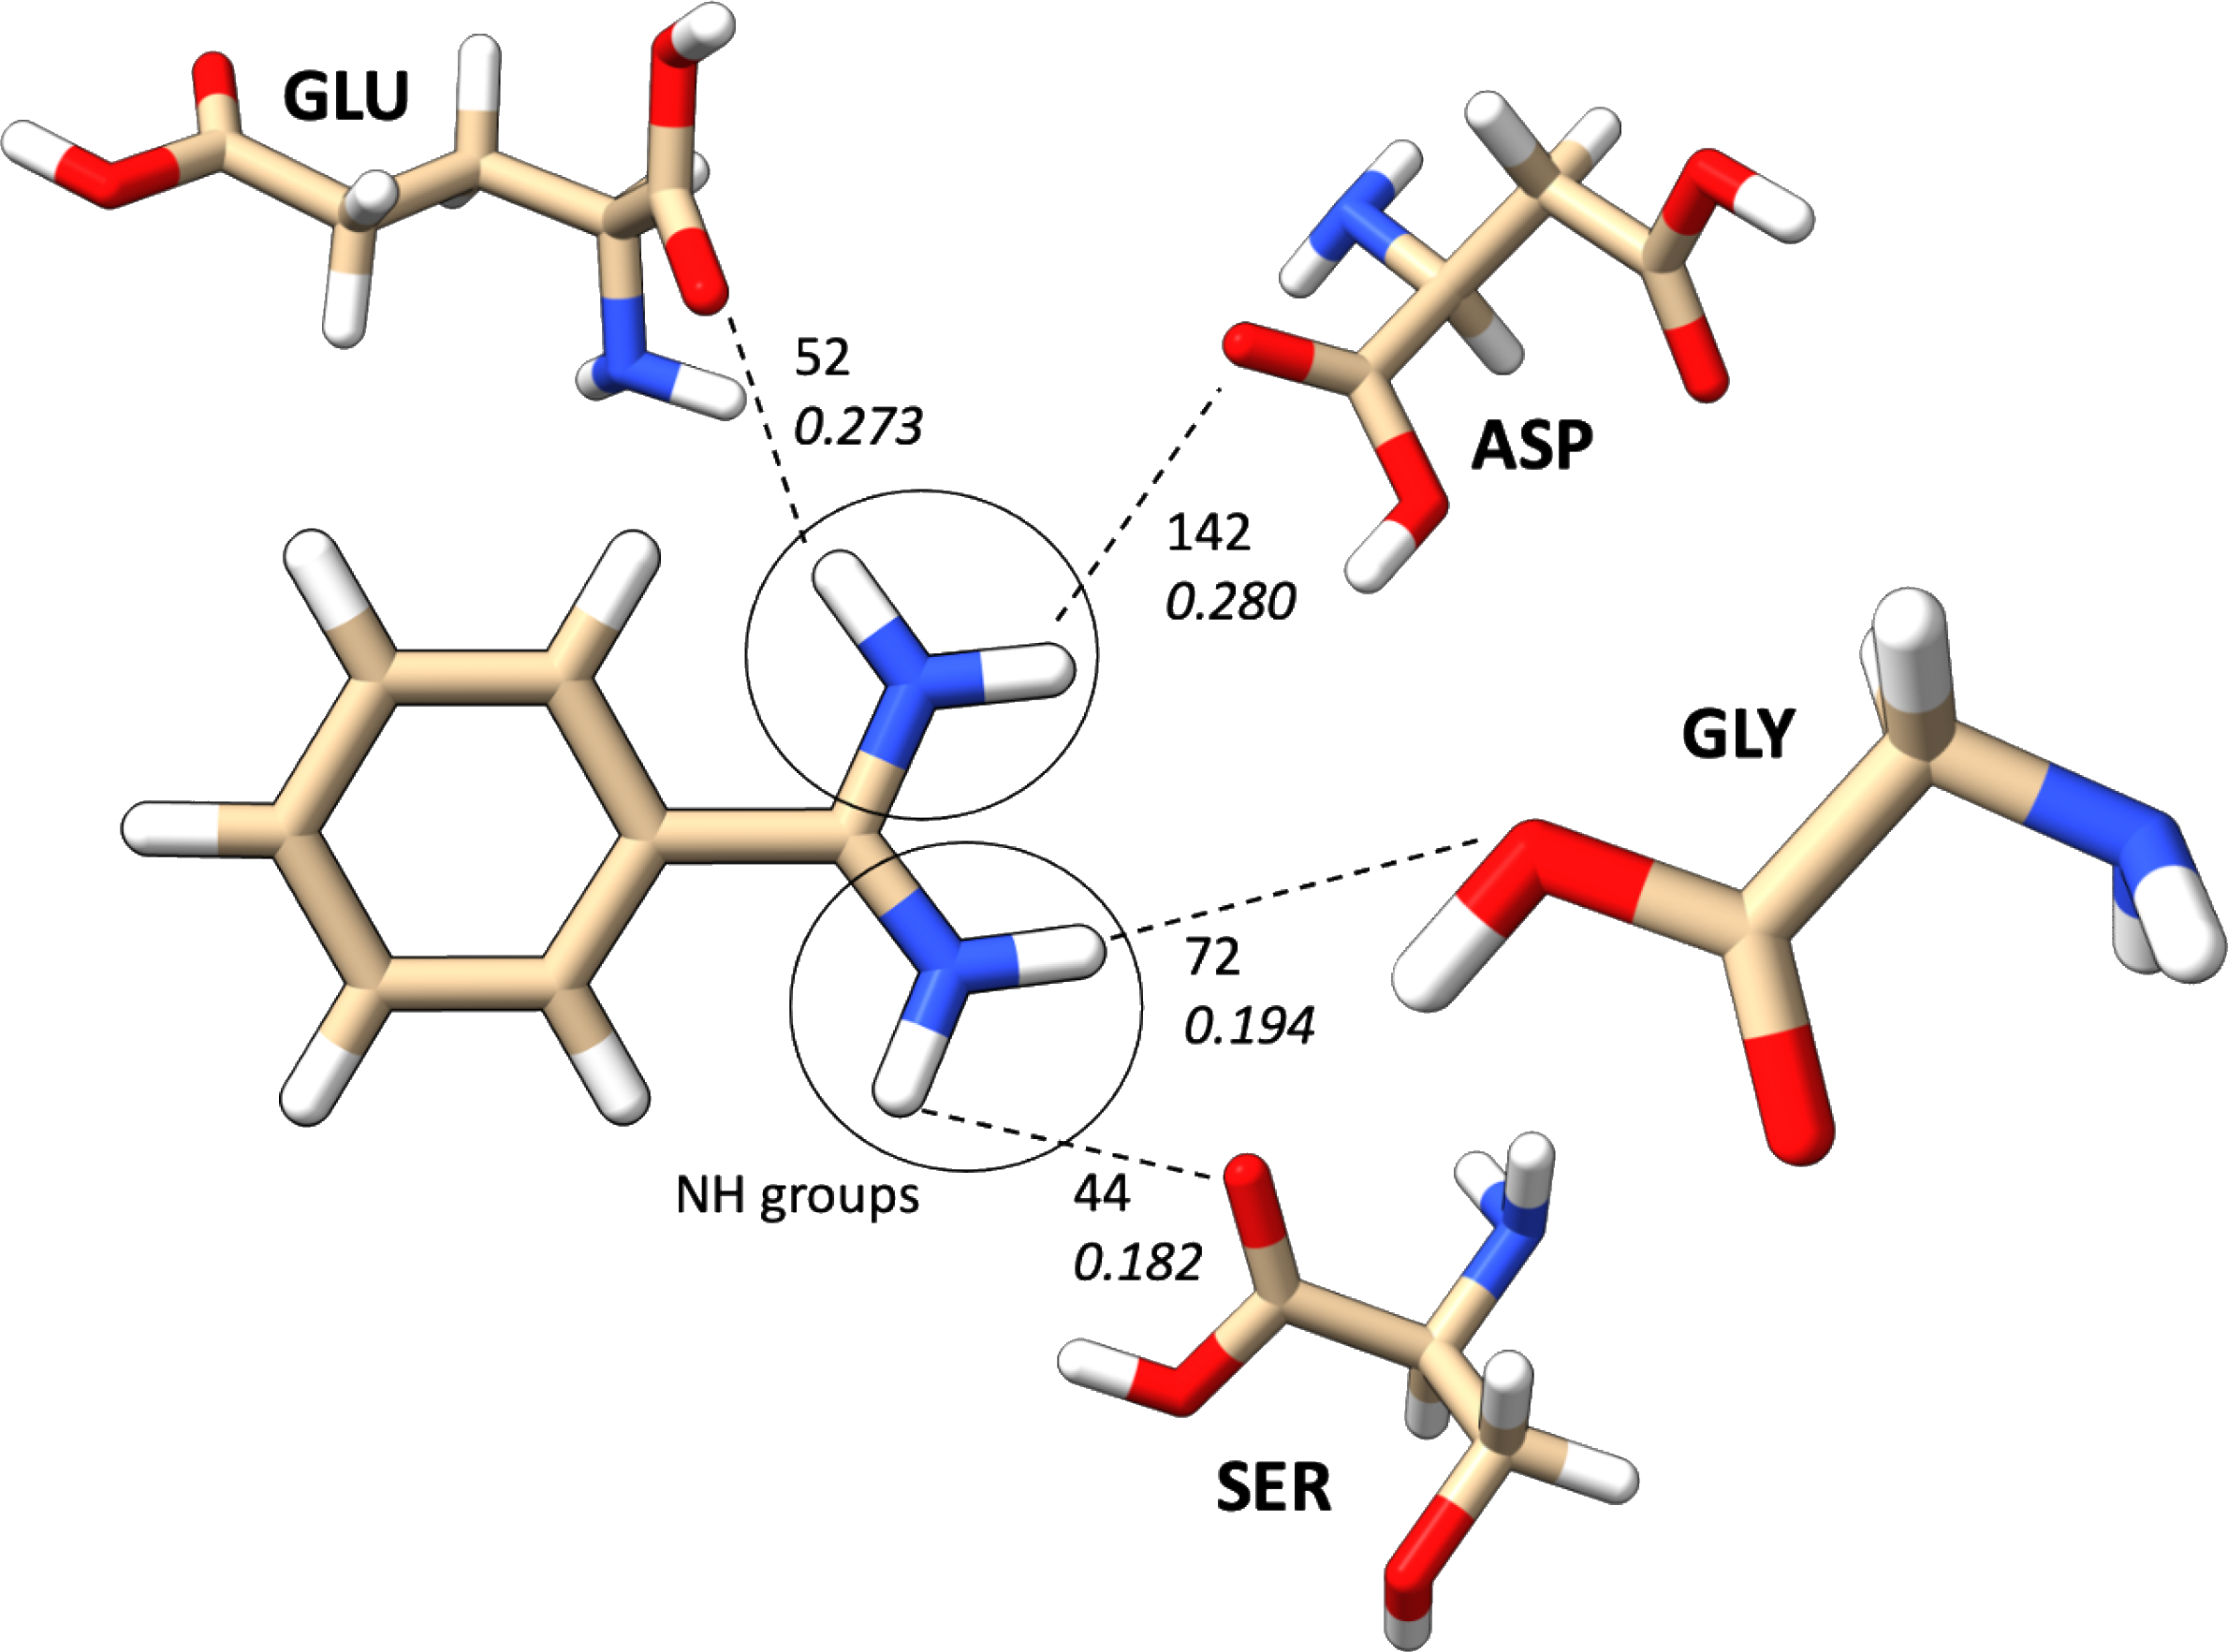
\includegraphics[width=0.5\textwidth]{figures/intro/hbonds.png}
      \caption{\label{fig:intro/hbonds} Hydrogen bond interactions between N-H groups acting as donors and oxygen atoms from aminoacids acting as receptors. Adapted from \cite{hbonds_2023}.}
    \end{figure}

    In proteins, oxygen and nitrogen atoms in both the backbone of the polypeptide and in the functional group of the aminoacids can act as donors or acceptors. The most common hydrogen bond interactions in proteins are of the form N-H...O, while O-H...O and N-H...N can also be commonly observed \cite{hbonds_2023}. In RNA, oxygen and nitrogen atoms in the nucleic bases take these roles (which sometimes leads to the notorious \textit{base pair} interaction) \cite{rna_2015} while oxygen atoms in the phosphate groups of their backbone could also act as acceptors in some cases \cite{hbonds_2023} (figure \ref{fig:intro/hbonds_po}).

    \begin{figure}[H]
      \centering
      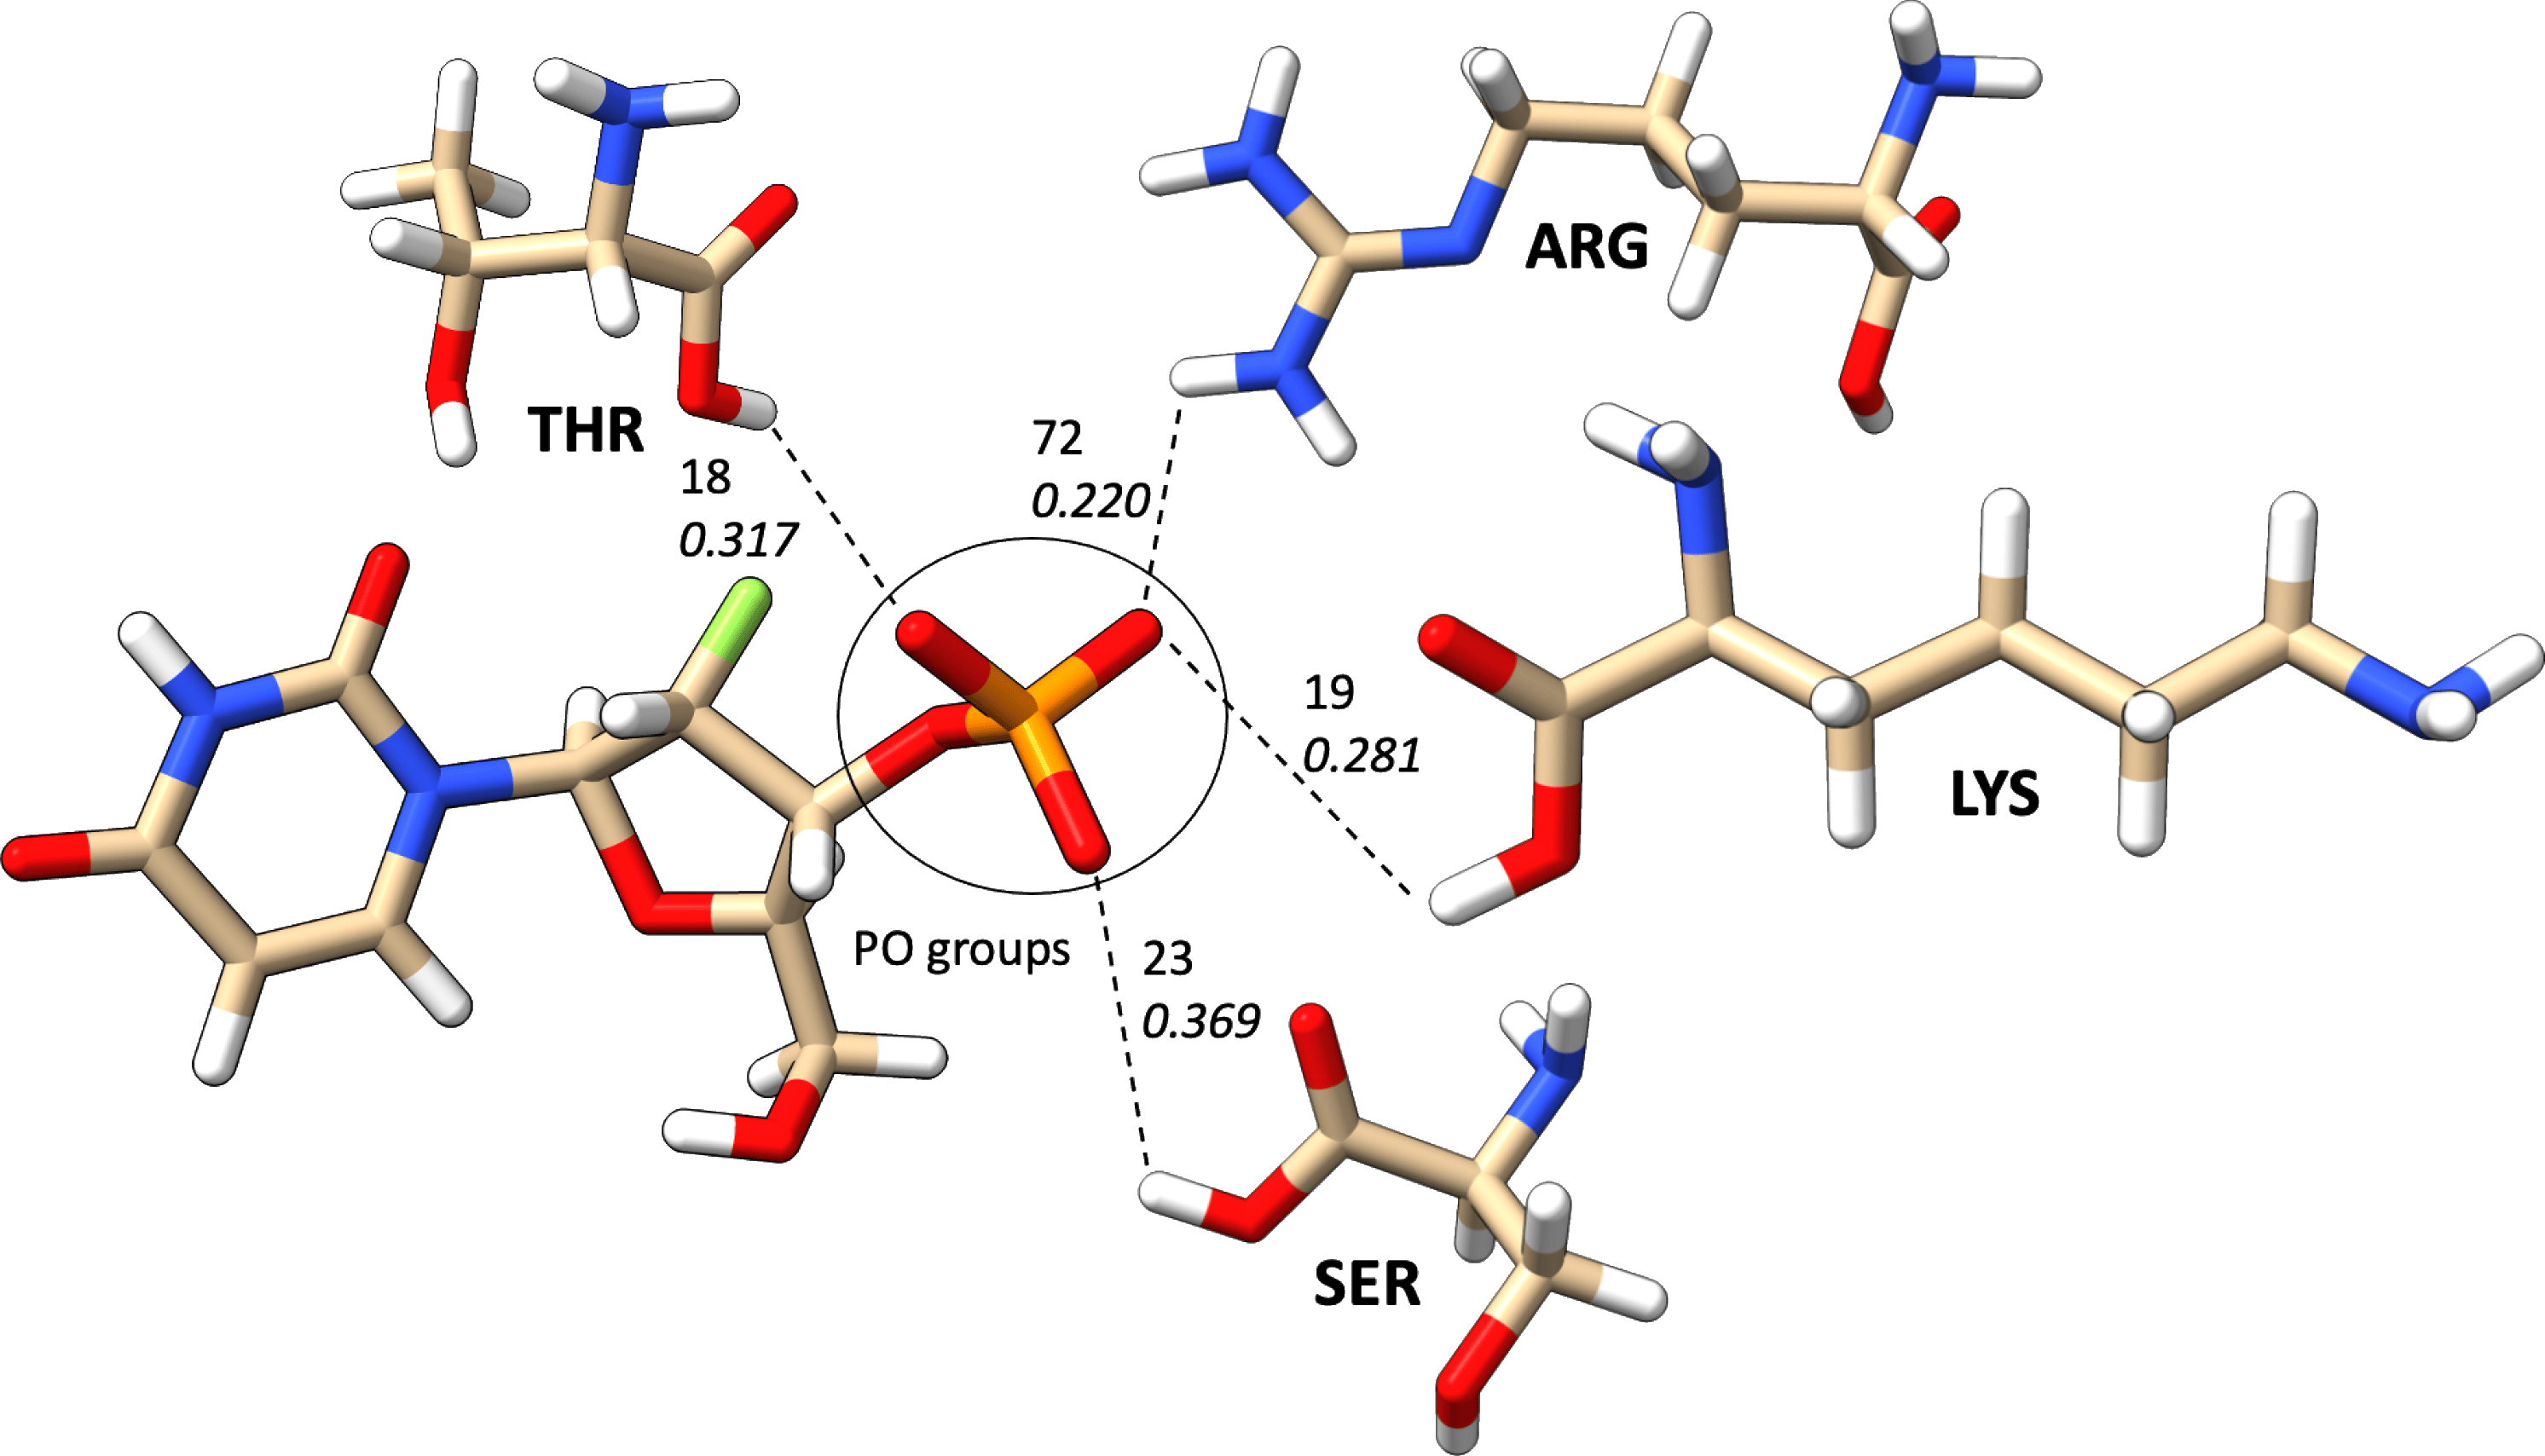
\includegraphics[width=0.5\textwidth]{figures/intro/hbonds_po.png}
      \caption{\label{fig:intro/hbonds_po} Hydrogen bond interactions between N-H and O-H groups acting as donors and a phosphate group acting as receptor. Adapted from \cite{hbonds_2023}.}
    \end{figure}

  \subsection{Hydrophobicity}
    The arrangement or displacement of water molecules near the surfaces of targets and ligands is also a very relevant factor that affects binding affinity \cite{hydrophobic_2017, hydrophobic_2022}. In structural terms, the dynamics of water can affect the structure and rigidity of the macromolecules, which sometimes affects the shape and flexibility of the pockets and therefore their binding affinity \cite{hydrophobic_2022}. In some instances, water is displaced from specific regions and energetically favorable interactions between non-polar groups emerge, which is commonly known as the \textbf{hydrophobic effect}. Hydrophobicity is mostly relevant in the case of some target proteins, where it is commonly associated to the formation of these \textit{solvent exclusion} (water displacement) cavities, usually buried inside the protein to avoid contact with the outside water (figure \ref{fig:intro/hydrophobic}) \cite{hydrophobic_2017}.

    \begin{figure}[H]
      \centering
      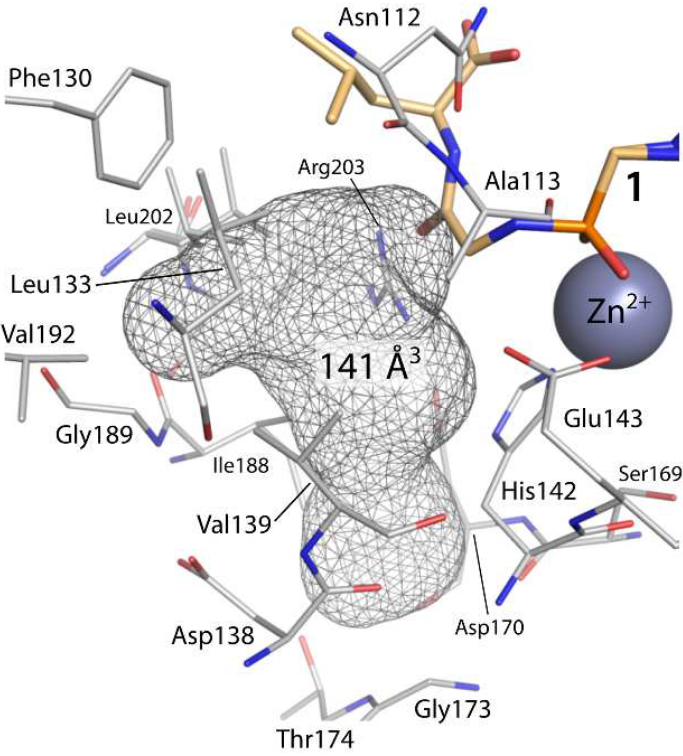
\includegraphics[width=0.5\textwidth]{figures/intro/hydrophobic.png}
      \caption{\label{fig:intro/hydrophobic} Volumetric representation of a solvent exclusion cavity inside of a metalloprotease (thermolysin). Adapted from \cite{hydrophobic_2017}.}
    \end{figure}


%%%%%%%%%%%%%%%%%%%%%%%%%%%%%%%%%%%%%%%%%%%%%%%%%%%%%%%%%%%%%%%%%%%%%%%%%%%%%%%%
\section{Molecular Visualization}
  \subsection{Molecular Visualization Software}
    Due to the nanoscopic nature of molecules, the field of molecular biology relies heavily on technologies to collect and gather insights from the structures and behaviour of these tiny systems. A great source of qualitative analysis and insight out of these data is enabled by the great variety of \textbf{molecular visualization software} and techniques that have been developed over the decades \cite{visualization_2018}.

    Molecular visualization is a huge topic constantly in evolution, with different parties developing different software packages or techniques to approach general or specific visualization purposes. Some of the most consolidated software environments are \textit{Chimera}, \textit{PyMOL}, \textit{PMV} and \textit{VMD} \cite{visualization_2018}. The Protein Data Bank lists a great variety of other software related to molecular graphics: \textit{BioBlender}, \textit{BioViz Studio}, \textit{CCP4mg}, \textit{Cn3D}, \textit{CrystalMaker}, \textit{ePMV}, \textit{EzMol}, \textit{Foldit}, \textit{ICM-Browser}, \textit{IcmJS}, \textit{iMol}, \textit{Jmol}, \textit{Mage and Kinemages}, \textit{Marvin}, \textit{MembraneEditor}, \textit{MOE}, \textit{Molecule World}, \textit{Molecules}, \textit{MolScript}, \textit{MolviZ.org}, \textit{Nanome}, \textit{PDBWORDS}, \textit{Perse Visualizer}, \textit{POLYVIEW}, \textit{Prosat}, \textit{Protein Imager}, \textit{QTree}, \textit{QuteMol}, \textit{RasMol}, \textit{Raster3D}, \textit{RasTop}, \textit{RCSB MBT Viewers}, \textit{RmscopII}, \textit{Schrödinger Product Suites}, \textit{SPADE}, \textit{STRAP}, \textit{Swiss PDB viewer}, \textit{UGENE}, \textit{WebMol}, \textit{YASARA}, \textit{Zeus} and \textit{ZMM} \cite{visualization_web}.

    Molecular visualization involves dealing with complex three-dimensional graphical data, oftentimes in a high-performant interactive way, which for large systems can be very computationally expensive. This challenge is shared with other fields in multimedia development, a notable one being the videogame industry. To take advantage of the highly optimized techniques used in videogame development, some molecular visualization tools have been built on top of \textit{game engines}. Tools such as \textit{UDock}, \textit{UnityMol} and \textit{CellVIEW} have been built using the notorious game engine \textit{Unity3D} \cite{visualization_2018, unitymol_2015, unitymol_web}.

    \begin{figure}[H]
      \centering
      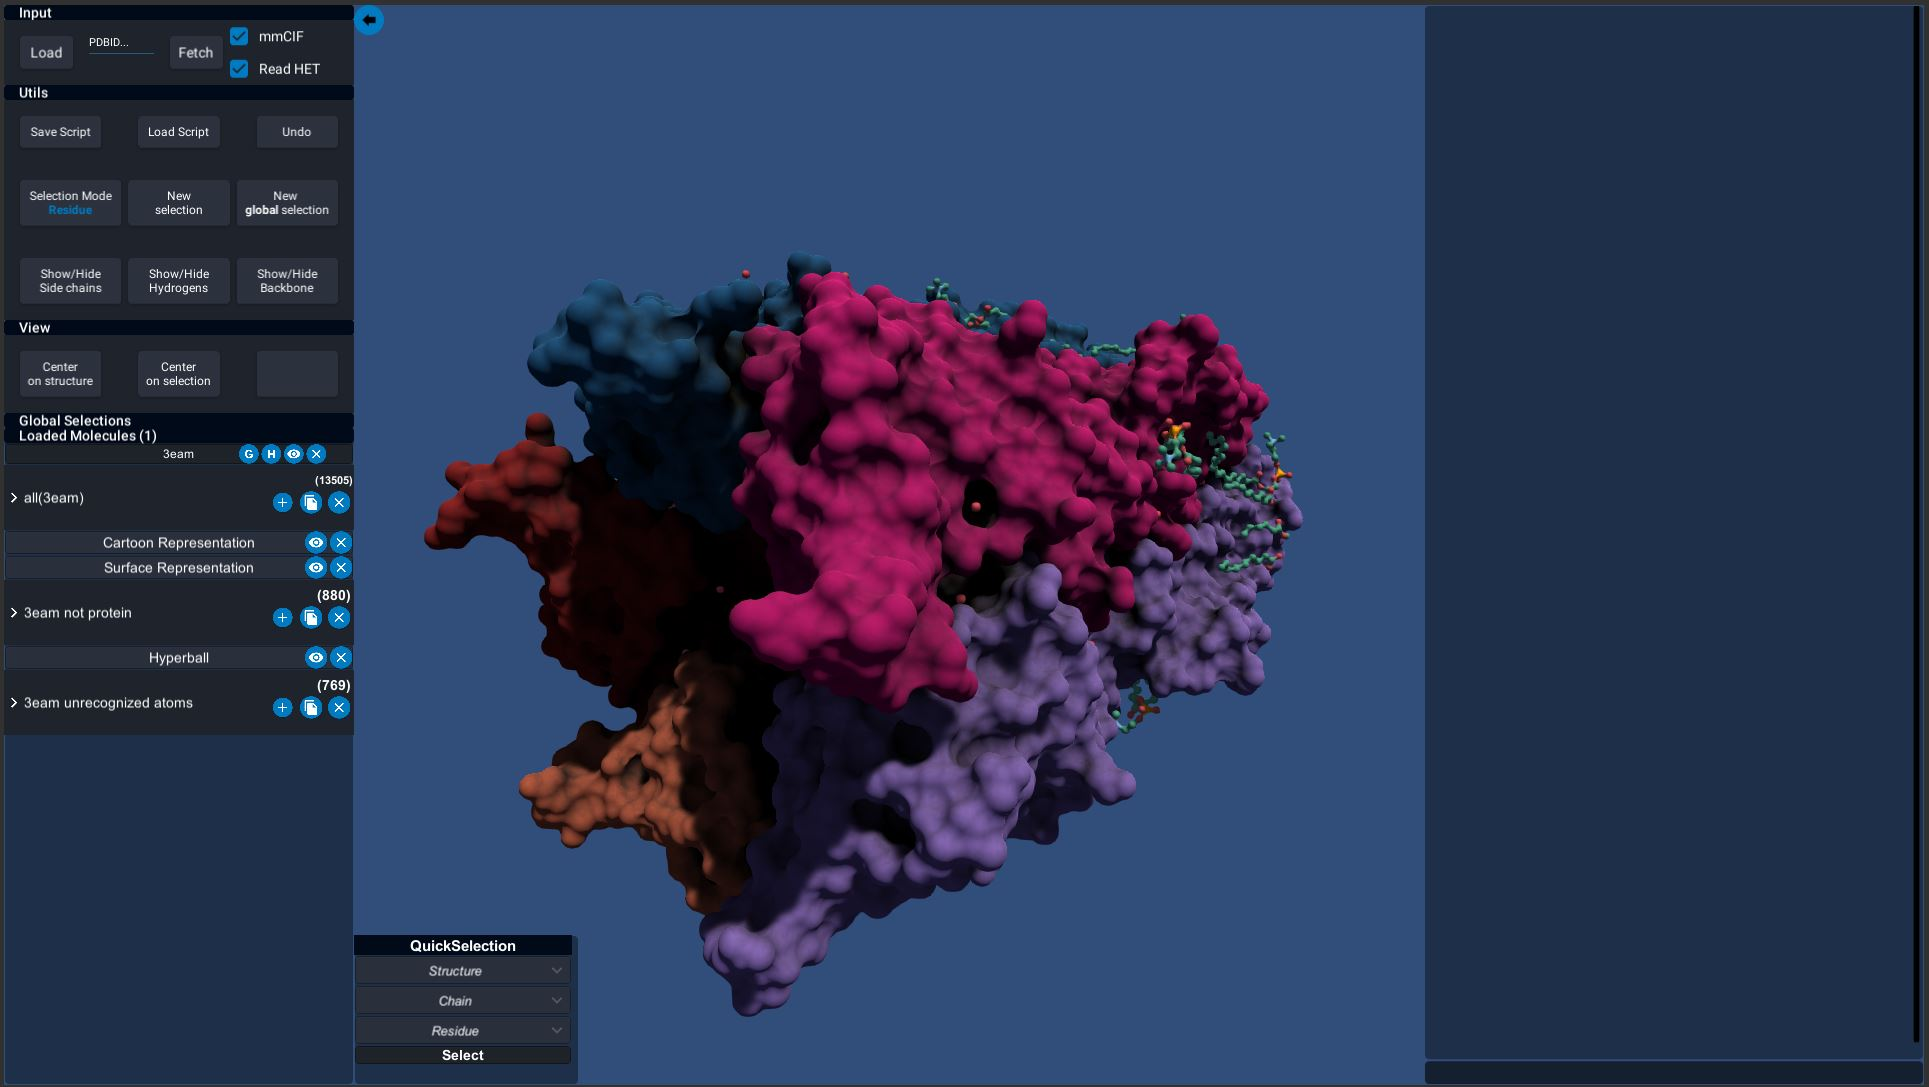
\includegraphics[width=0.5\textwidth]{figures/intro/unitymol.jpg}
      \caption{\label{fig:intro/unitymol} Visualization of a protein interacting with ligands using UnityMol. Adapted from \cite{unitymol_web}.}
    \end{figure}

    The molecular viewer \textbf{UnityMol} covers the basic functionalities of molecular visualization (figure \ref{fig:intro/unitymol}), while also serving as an environment for prototyping new representation techniques for specific systems or properties. It can be used to visualize proteins, nucleic acids, polysaccharides, ligands, molecular dynamics trajectories, among others. It also takes advantage of graphical and computational resources provided by the engine, such as shader GPU programs (for optimized structure representations) and the VRTK framework (for developing a \textit{virtual reality} approach to molecular visualization) \cite{unitymol_2015, unitymol_web}.

  \subsection{Molecular Representations}
    Molecular visualizers employ different data visualization techniques to portray the structural and physicochemical information of the biological systems in an intuitive and ergonomic way. Visual cues are exploited for this purpose, such as shapes, contours, color-codes, opacities, labels, animations (in the case of molecular dynamics trajectories), among others. These tecnhiques allow to build \textbf{representations} of the molecules, called this way because they seek to represent the spatial three-dimensional data into an intuitive and tangent object that can be observed and interacted with. Classical examples of representations include \textit{ball and stick}, \textit{cartoon}, \textit{licorice}, \textit{line}, \textit{point}, \textit{ribbon}, \textit{rocket}, \textit{spacefill}, \textit{surface} and \textit{trace} (note that names can change on different software implementations) \cite{representations_web}. Insightful observations can be obtained by alternating between this representations in different parts of a molecular system of interest.

    \begin{figure}[H]
      \centering
      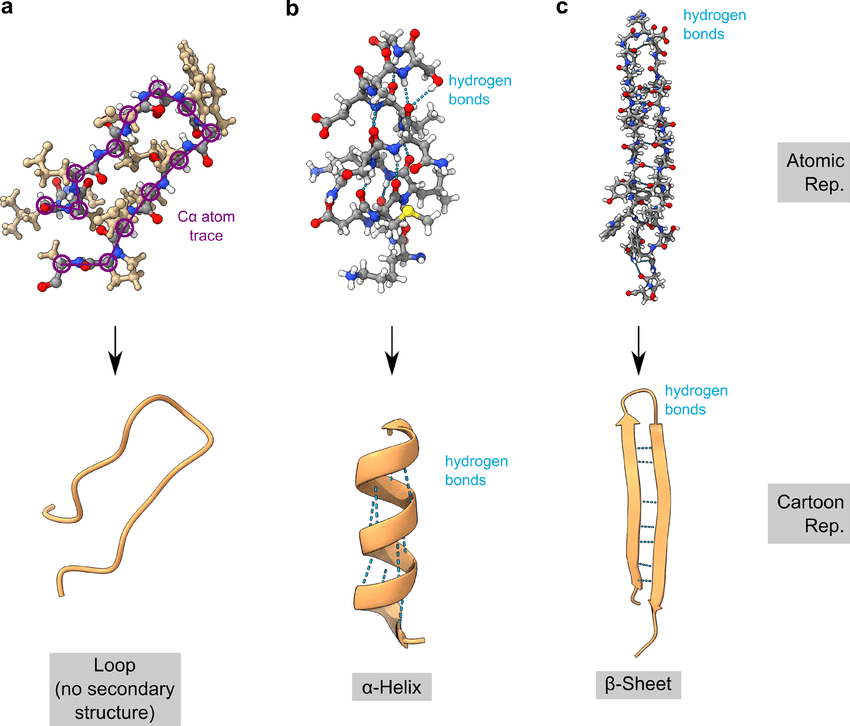
\includegraphics[width=0.5\textwidth]{figures/intro/rep_cartoon.png}
      \caption{\label{fig:intro/rep_cartoon} [TODO] description. Adapted from \cite{representations_2021}.}
    \end{figure}

    The \textbf{licorice} representation highlights the \textit{bond topology} of the molecules and is often color coded according to each atom, so it is best suited for small molecule ligands or closeups of pocket structures (figures \ref{fig:intro/pocket}, \ref{fig:intro/pharmacophores}, \ref{fig:intro/electrostatics}, \ref{fig:intro/hbonds}, \ref{fig:intro/hbonds_po}, \ref{fig:intro/hydrophobic}, \ref{fig:intro/unitymol}, \ref{fig:intro/rep_cartoon}, \ref{fig:intro/rep_surfaces}). The \textbf{cartoon} representation summarizes the \textit{secondary structure} of macromolecules into simpler shapes. This is usually associated to proteins (figures \ref{fig:intro/rep_cartoon}, \ref{fig:intro/rep_surfaces}) but can also be applied to nucleic acids, polysaccharides, lipids and other macromolecules.

    For the \textbf{surface} representations, the volume occupied by the electronic clouds of the atoms is estimated by an algorithm, then a contour is drawn around this volume to obtain a tangible shape that emphasizes the overal \textit{three-dimensional shape} of the molecule (figures \ref{fig:intro/pocket}, \ref{fig:intro/electrostatics}, \ref{fig:intro/unitymol}, \ref{fig:intro/rep_surfaces}). More or less precise algorithms can be used to calculate this estimation, depending if precision or performance is to be prioritized. Alternatively, a \textbf{spacefill} representation can be employed, where a sphere is drawn around each atom with a theoretical radius that depends on the element (figures \ref{fig:intro/hydrophobic}, \ref{fig:intro/rep_surfaces}).

  \subsection{Visualization of Physicochemical Properties}
    Apart from the spatial configuration of the molecules, the physicochemical properties of the system are also of interest for many applications, such as protein-ligand interactions. As such, the visualization of these data should also be considered when developing molecular visualizers. The \textbf{electrostatics} of the molecules is usually portrayed by color-coding surface representations, where different colors correspond to different sign and intensity of surface charges (figures \ref{fig:intro/electrostatics}, \ref{fig:intro/rep_surfaces}). Similarly, \textbf{hydrophobicity} is many times represented also by color-coding the surfaces of the molecules, according to theoretical or empirical hydrophobic qualities of the residues or functional groups involved (figure \ref{fig:intro/rep_surfaces}).

    \begin{figure}[H]
      \centering
      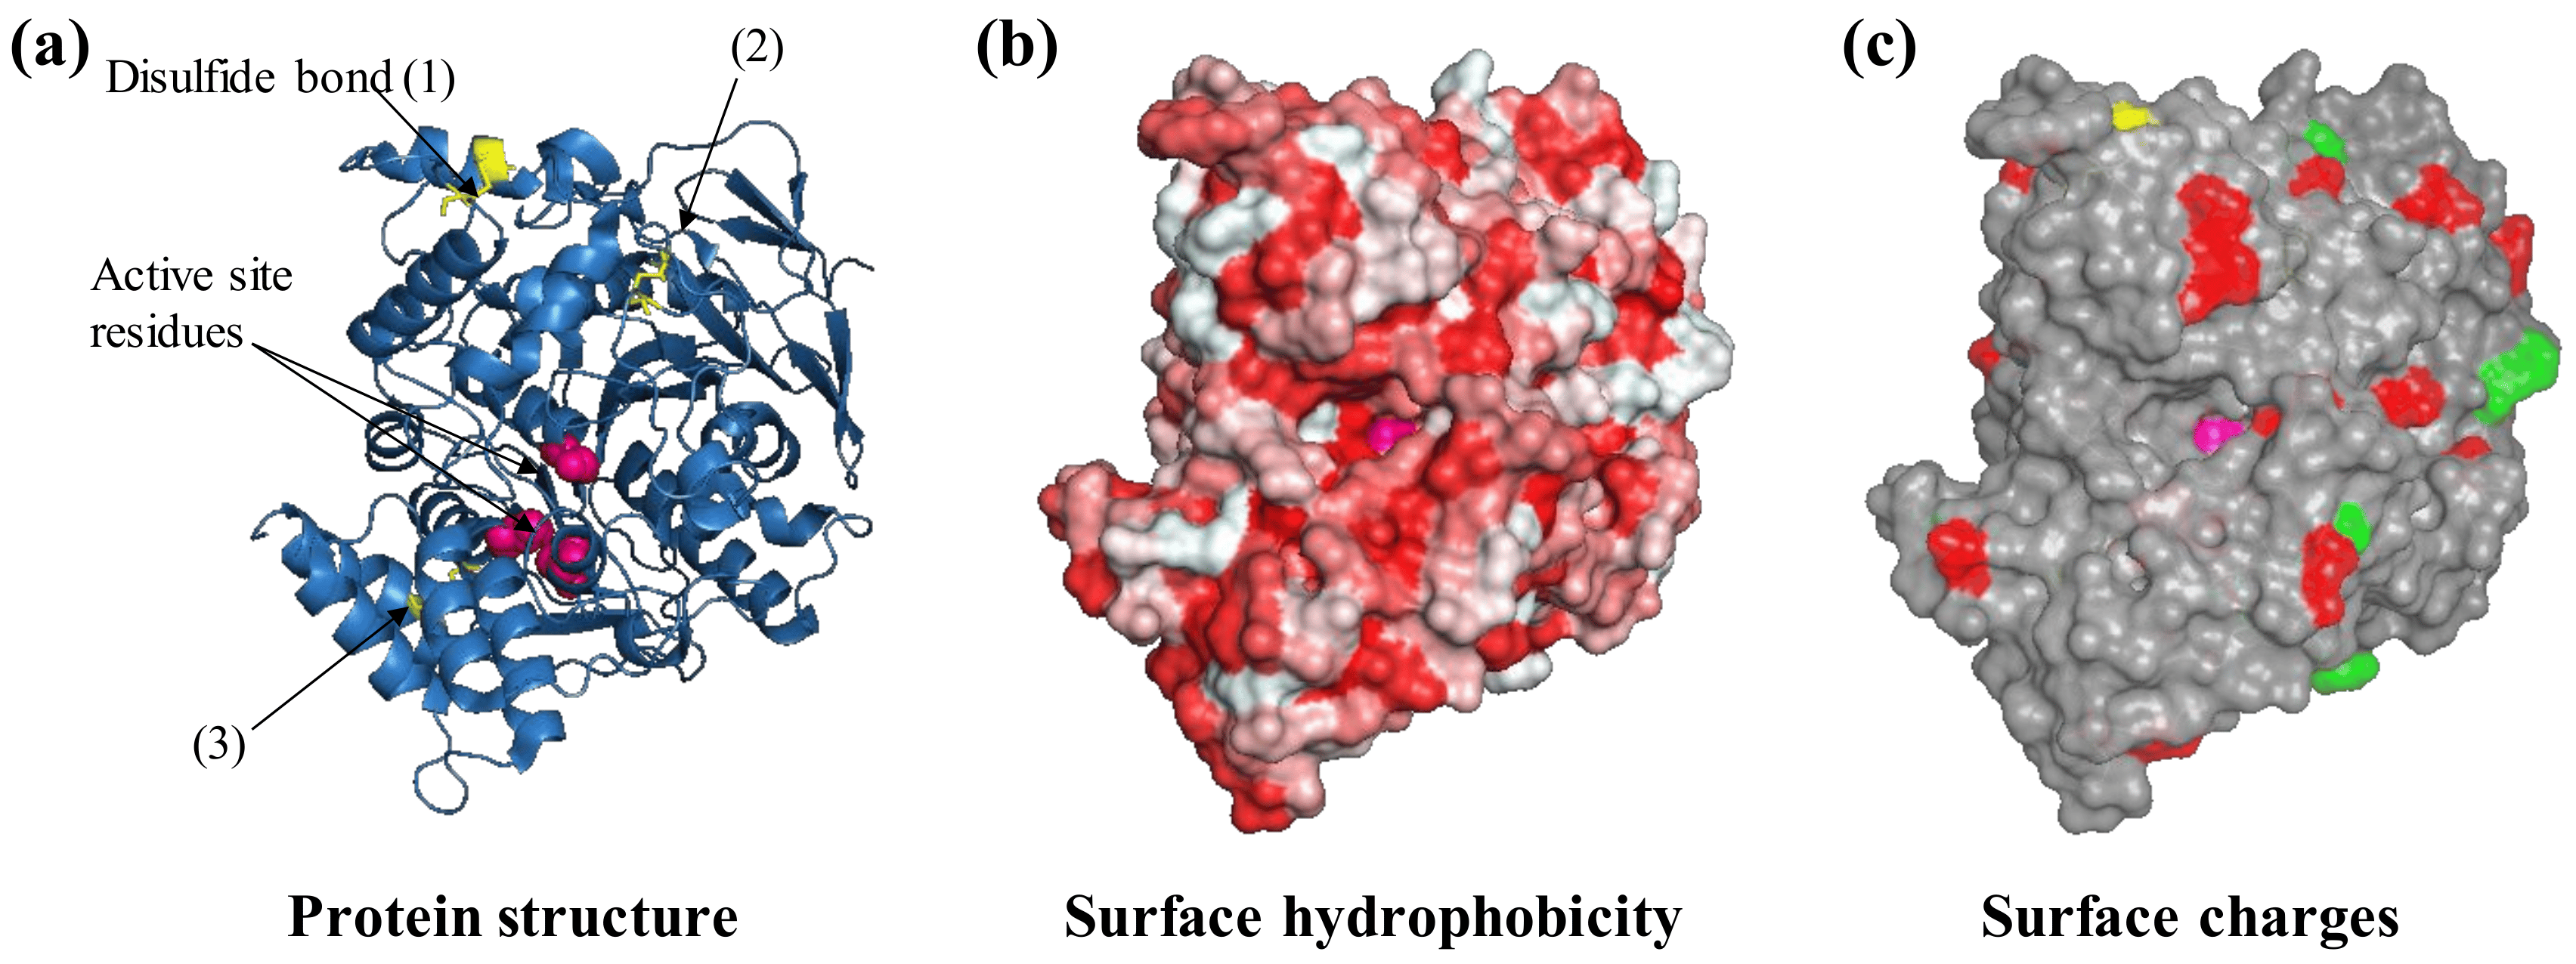
\includegraphics[width=0.5\textwidth]{figures/intro/rep_surfaces.png}
      \caption{\label{fig:intro/rep_surfaces} [TODO] description. Adapted from \cite{representations_2018}.}
    \end{figure}

    In the case of \textbf{hydrogen bonds}, the common approach is to represent them as dotted lines between the acceptor and donor atoms (figures \ref{fig:intro/hbonds}, \ref{fig:intro/hbonds_po}, \ref{fig:intro/rep_cartoon}). On the other hand, \textbf{stacking} interactions are not usually represented in any particular way. Instead, visualizers rely on the users to observe the proximity and positioning between aromatic rings and judge in an approximate manner whether stacking can be present or not.

    Interestingly, visualizers tend to focus on \textit{surface} representations when displaying physicochemical properties. However, some of these properties are inherently \textit{volumetric}, such as electrostatics and hydrophobicity. Also, when studying pocket-ligand interactions, pharmacophores further encapsulate hydrogen bonds and stacking as elements that occupy a volume of propensity. Indeed, the volume surrounded by the target pocket can be considered to contain the physicochemical properties required to study and design target-ligand interactions, but this is not exploited much in current molecular visualization.

    \begin{figure}[H]
      \centering
      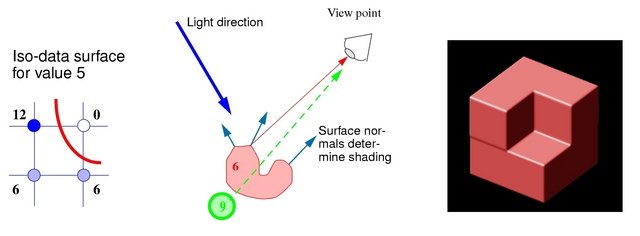
\includegraphics[width=0.5\textwidth]{figures/intro/isosurfaces.png}
      \caption{\label{fig:intro/isosurfaces} [TODO] description. Adapted from \cite{isosurfaces_web}.}
    \end{figure}

    A notable exception is the use of a volumetric representation known as \textbf{isosurface}. This technique for visualizing three-dimensional grids of data use an adjustable treshold value to draw a contour around points with similar values, which yields a representation similar to a \textit{surface} one (figure \ref{fig:intro/isosurfaces}) \cite{isosurfaces_web}. Isosurfaces are sometimes used to represent solvent exclusion cavities when studying the hydrophobicity of a system (figure \ref{fig:intro/hydrophobic}).


%%%%%%%%%%%%%%%%%%%%%%%%%%%%%%%%%%%%%%%%%%%%%%%%%%%%%%%%%%%%%%%%%%%%%%%%%%%%%%%%

  %%% summarize the project rationale, the scientific hypothesis and the key experiments that have been planned to test the hypothesis
\chapter{Objectives} % at least 1 page, not more than 2 pages

[TEMPLATE: summarize the project rationale, the scientific hypothesis and the key experiments that have been planned to test the hypothesis.]

  %%% detailed description of the protocols, software and algorithms used for the project
\chapter{Materials and methods} % at least 3 pages, maximum 10 pages

%%%%%%%%%%%%%%%%%%%%%%%%%%%%%%%%%%%%%%%%%%%%%%%%%%%%%%%%%%%%%%%%%%%%%%%%%%%%%%%%
\section{Computational environments}
  All the calculations and data handling required for the modelling and potential calculations were performed using \textbf{Python} version 3.10.5 \cite{python_2009}. Even if it is not the most performant option, its flexibility and seamless syntaxis allow for quick experimentation when developing the models; it is well known for its powerful data visualization packages, such as \textbf{Matplotlib} \cite{python_2021}. Nevertheless, the performance of the calculations was optimized by employing the package \textbf{NumPy} for parallelizable matrix computations \cite{numpy_2020}, \textbf{pandas} for data manipulation \cite{pandas_2020} and multiprocessing techniques from the standard library.

  Furthermore, for parsing PDB files, the Python package \textbf{MDAnalysis} (MDA) is used \cite{mda_2016, mda_2011}. This package allows for selecting specific atoms of the system by means of a query, which is useful for performing operations using only the atoms of interest. Matrices with values for the potentials are stored using the \textbf{JSON} \cite{json_web} and \textbf{DX} \cite{opendx_web} specifications.

  The visualization software \textbf{VMD} \cite{vmd_96} was used as a reference points for testing with queries for molecular selections, representations and other aspects of the pipeline. All new molecular visualization and user interaction procedures where developed in \textbf{UnityMol} \cite{unitymol_web}, by employing the GUI-based development workflow provided by \textbf{Unity3D}. Necessary scripts were written using the language \textbf{C\#}, as required by the engine \cite{unity_2014}.


%%%%%%%%%%%%%%%%%%%%%%%%%%%%%%%%%%%%%%%%%%%%%%%%%%%%%%%%%%%%%%%%%%%%%%%%%%%%%%%%
\section{Characterization of Physicochemical Properties}
  \subsection{Stacking Potential}
    \subsubsection{Obtaining the Datasets}
      For modeling the stacking potential, the shape and parameters of a statistical energy function were empirically determined. A large dataset of protein, protein/ligand, protein/nucleic and protein/nucleic/ligand systems was downloaded from the Protein Data Bank (PDB) \cite{pdb_2003}. First of all, the PDB ids for these systems were obtained by submitting two queries to the database:

      \begin{itemize}
        \item \textbf{For protein and protein/ligand}: \textcolor{teal}{"entry polymer types = protein only" \& "number of assemblies = 1" \& "experimental method = X-ray diffraction" \& "data collection resolution < 2.5 \AA"}
        \item \textbf{For protein/nucleic and protein/nucleic/ligand}: \textcolor{teal}{"entry polymer types = protein/NA" \& "number of assemblies = 1" \& "experimental method = X-ray diffraction" \& "data collection resolution < 2.5 \AA"}
      \end{itemize}

      These PDB ids were used to programatically download the dataset by means of bash scripts and interacting with the PDB's API. Then, a Python script was employed for extracting ligand names from the PDB files. These names were similarly used for downloading a dataset of CIF ligand description files from PDB.

    \subsubsection{Detecting Aromatic Groups in Ligands}
      For parametrizing this model, only ligands with aromatic groups are of interest. A first approach for filtering the ligands was to parse the SMILES string from the CIF files and keep only those that contained flags for presence of aromatic bonds (i.e. lowercase letters).

      After some issues with the first method, a second approach was also deviced. A Python script was used for inspecting the bonds topology described in the CIF files. A ligand was considered to be candidate for aromaticity if its structure had cycles after discarding tetrahedral atoms (i.e. those with four bonds). In this case, information about the individually detected cycles was stored in a CSV file.

      Ligands where the two methods coincided were considered to have an aromatic group for the next steps. Cases where the methods disagreed were manually inspected to decide whether to consider them aromatic or not.

    \subsubsection{Coarse-grained Description of Aromatic Groups}
      Before sampling the aromatic interactions, all aromatic groups are simplified into a coarse-grained description. For each aromatic group, a particle is defined at the \textbf{center of geometry} (COG) of the group (i.e. the average position of the atoms that conform it). In cases where an aromatic group is made by two adjacent aromatic rings (such as tryptophan or adenine), the center of geometry of the whole group is considered as a single point. The \textbf{normal vector} of the aromatic plane (i.e. the three-dimensional vector perpendicular to the plane) is also calculated for each group (figure \ref{fig:methods/aromatic}).

      \begin{figure}[H]
        \centering
        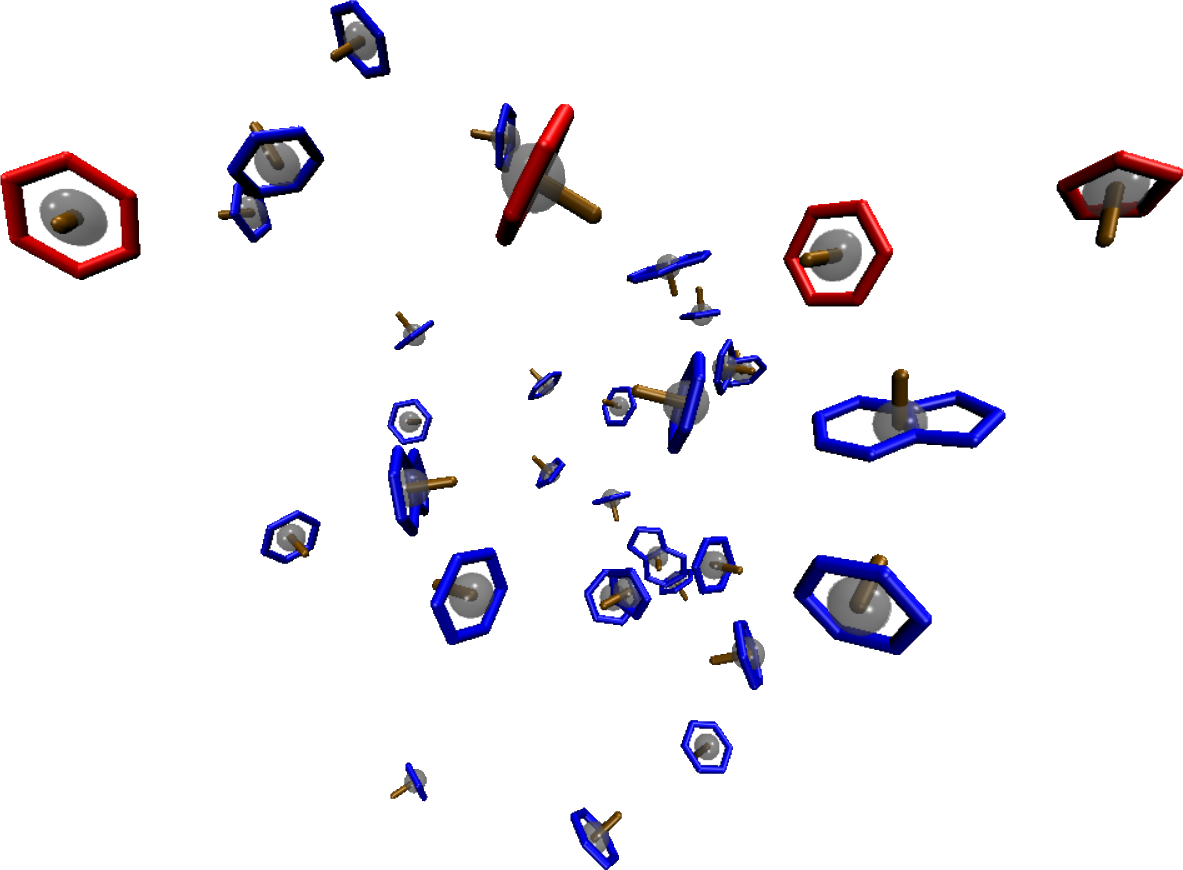
\includegraphics[width=0.5\textwidth]{figures/methods/aromatic.png}
        \caption{\label{fig:methods/aromatic} Aromatic groups and their coarse grained representation. Blue) aminoacid aromatic rings, Red) nucleic acid aromatic rings, Silver) center of geometry, Bronze) normal vector. PDB: 1IQJ.}
      \end{figure}

      Atoms corresponding to aromatic groups are selected by a query that specifies the aromatic residue names and the specific atom names that compose their aromatic rings. This information is stored in lookup tables, which are straightforward in the case of amino and nucleic acids, although \textit{synonyms} must be covered (i.e. a residue having more than one possible name, such as adenine been identified as \textbf{A} or \textbf{ADE} in different PDB files).

      Additionally, some synonyms used by MDA for amino or nucleic acids are actually used by PDB for unrelated ligands (for example \textbf{THY} refers to thymine according to MDA but to a ligand according to PDB). This ligand information is stored in the look up tables just for good measure. Finally, the look up table for the ligands is simply the curated CSV file obtained from the ligand dataset in the previous step. Note that, whenever a ligand has more than one separate aromatic group in their structure, each group is reported as a separate row. The lookup tables employed for protein (table \ref{tab:methods/aromatic_prot}), nucleic (table \ref{tab:methods/aromatic_nucleic}) and the first twenty rows for ligands (table \ref{tab:methods/aromatic_ligand}) are available at Appendix I.

    \subsubsection{Sampling of Aromatic Interactions}
      Two aromatic groups were considered to interact when their corresponding coarse-grained particles where under a certain distance range, set to be between {3 \AA} and {6.5 \AA} following the observations of similar data analysis studies \cite{aromatic_2018}. To obtain all aromatic interactions present in a PDB file, an all-to-all pairwise confrontation was done between the aromatic groups of the system. For those under the spatial proximity of interest, the distance and the $\alpha$ and $\beta$ angles were calculated.

      Note that, given two particles $i$ and $j$, the distance and $\beta$ values are the same for the $i-j$ and $j-i$ interactions, however the $\alpha$ values my differ between $i-j$ and $j-i$. Therefore, for each pair of aromatic groups, two interaction datapoints are produced, with duplicate distance and $\beta$ values and possibly unique $\alpha$ values. This process was performed over the entire dataset of PDB files, employing multithreading to speed up the process.

    \subsubsection{Model Definition}
      After filling the interactions dataframe, standard data visualization techniques were performed to observe how the distance, $\alpha$ and $\beta$ values interacted. Observing the histograms obtained from these data allowed for extracting an empirical shape and parameters for the distribution of stacking interactions, needed for defining the stacking potential model.

  \subsection{Hydrogen Bonds Potential}
    Theoretically, modeling hydrogen bond interactions depends on the distances and angle between acceptor, donor and the hydrogen atom. However, when generating a statistical potential field, only acceptor or donor+hydrogen are available, as by definition the potential field is built to estimate the most probable configurations for the missing second half of the interaction. This means that, if the potential field is built without introducing simplifications, it would require a four dimensional space (three spatial dimensions plus the \textit{hydrogen bond angle} dimension) to properly describe the interaction.

    Therefore, for modeling the hydrogen bond interactions, an assumption is made that only hydrogen bonds with an ideal angle of approximately $180^{\circ}$ are considered. The model is further simplified by neglecting the position of any hydrogen atoms in the PDB structure, based in the idea that usually the positions of the hydrogen atoms vary much fast than that of the donor atoms, which means it is better to base the model only on where the donors and acceptors might be.

    With this in mind, the hydrogen bond potential model was defined as a \textbf{sum of univariate normal distributions} centered in the acceptor and donor atoms of the structure of interest. The only parameter considered by the model was the distance from any given acceptor or donor atom to any point in the three-dimensional space. The parameters for the probability distribution are $\mu = 3$ and $\sigma = 0.15$ [TODO: cite?].

  \subsection{Electrostatic Potential}
    Quantifying the electrostatic potential around atoms of a molecular system overlaps smoothly with the functionality of the APBS software. Hence, there is no need to model the interaction potential in this case and it is enough to incorporate the APBS pipeline into the workflow. However, there might be issues in the visualization stage with the fact that this potentials can vary significantly in magnitude (figure \ref{fig:methods/lapbs}.0).

    \begin{figure}[H]
      \centering
      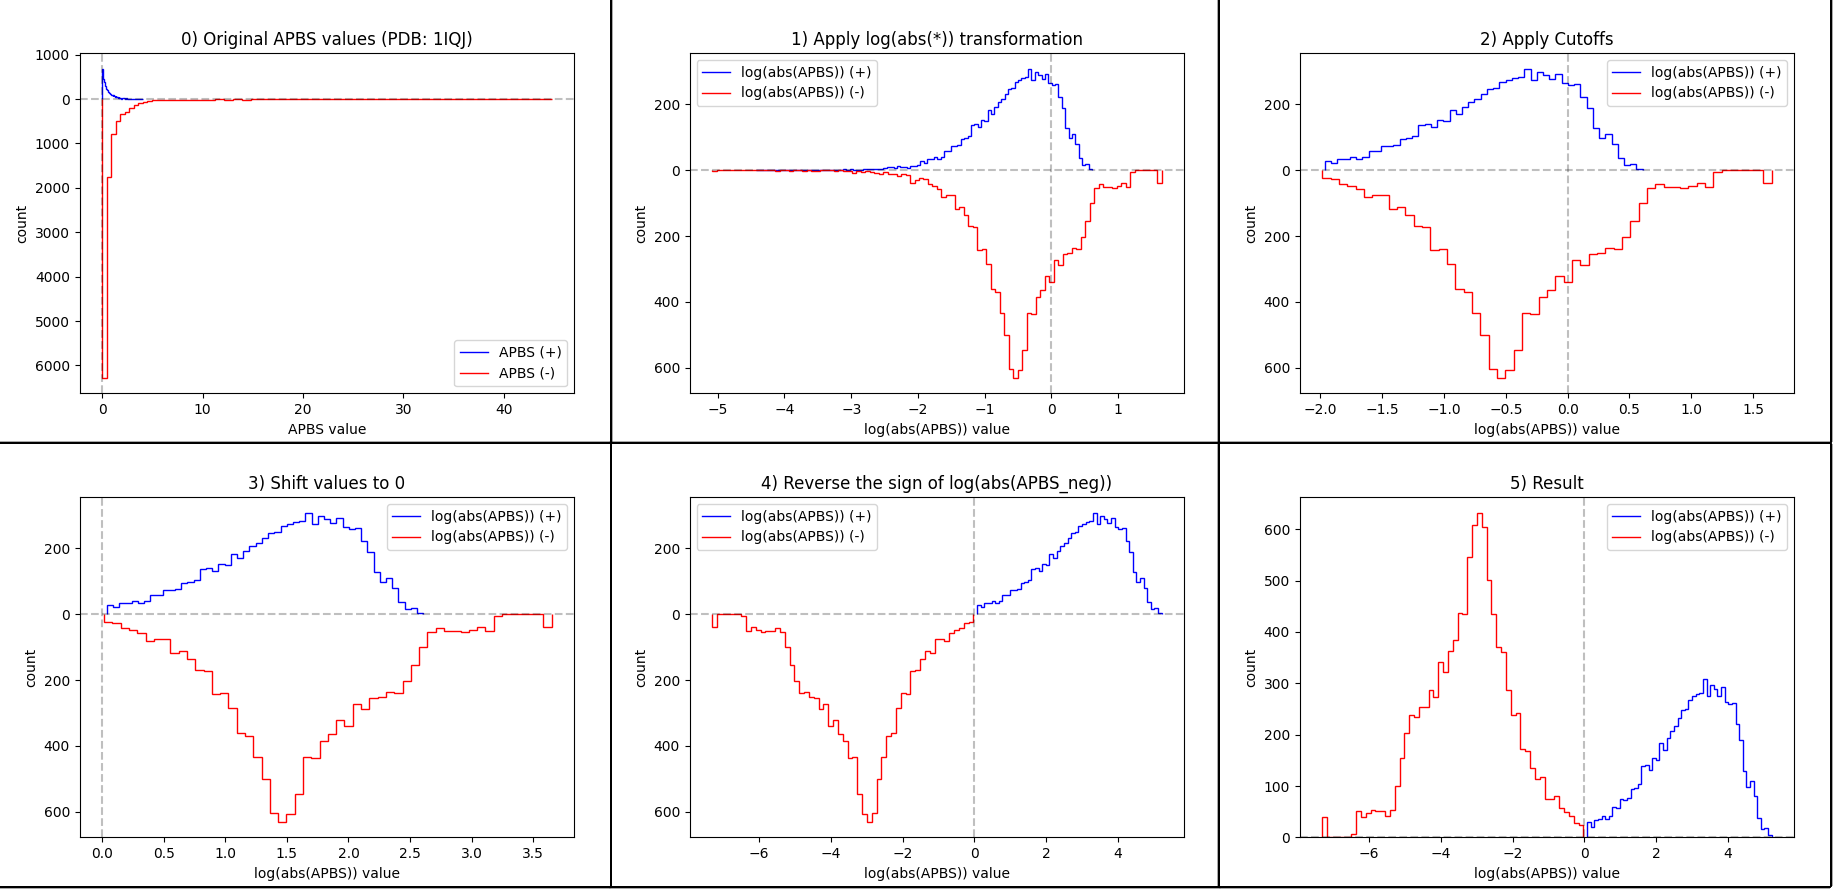
\includegraphics[width=1\textwidth]{figures/methods/lapbs.png}
      \caption{\label{fig:methods/lapbs} [TODO: description, transpose image source? (2x3 layout instead of 3x2)]}
    \end{figure}

    Although moving the values into the logarithmic scale is the intuitive solution for this problem, it can not be done in a straightforward way, as the model  calculates actual physical values related to the charges of the system (instead of propensity values as in the previous cases) which can also be negative. To avoid negative values, the absolute value of the points is taken before applying the logarithm base 10 (figure \ref{fig:methods/lapbs}.1).

    By applying this transformation, negative and positive values are obtained, which this time represent the \textit{scale} of the quantities instead of their \textit{physical} meaning; it is evident however that both are important to conserve. To achieve this, the transformed set of points is first pruned to conserve only meaningful and common values. This is done by applying two empirical cutoffs: a minimum of $-2$ and a maximum of $3$ (figure \ref{fig:methods/lapbs}.2) This procedure fixes the boundaries for the points, which in turn allows to shift their origin to 0 by substracting the value of the lower boundary (figure \ref{fig:methods/lapbs}.3).

    Now that all points are positive and the scale information is still conserved, it is time to bring back the physical meaning of signed electrostatic potential. To achieve this, the points that originally corresponded to negative APBS values are simply multiplied by $-1$ to reverse their sign (figure \ref{fig:methods/lapbs}.4). In this step, all points are also scaled by a factor of $2$, with the purpose of having the boundaries at a fixed $[-10, 10]$ range, and the points neatly normalized in between (figure \ref{fig:methods/lapbs}.5).

  \subsection{Hydrophobicity Potential}
    The hydrophobicity potential was modelled in a similar way to the hydrogen bonds, as a sum of univariate normal distributions centered around every atom of interest. The parameters for the probability distribution are $\mu = 3.7$ and $\sigma = 0.15$ [TODO: cite?]. Each distribution is scaled by a hydrophobicity value, which depends on the type of residue from which the atom is part of. For aminoacids, these values correspond to the Kyte-Doolittle scale, which uses positive values to represent hydrophobic residues and negative values for hydrophilic. On the other hand, this model was not implemented for RNAs, due to their mostly hydrophilic nature.


%%%%%%%%%%%%%%%%%%%%%%%%%%%%%%%%%%%%%%%%%%%%%%%%%%%%%%%%%%%%%%%%%%%%%%%%%%%%%%%%
\section{Development of Visualization Methods}
  \subsection{Graphical User Interface}
    A menu component was built for the Graphical User Interface (GUI) of UnityMol, to allow for an easy interaction between the user and the potentials calculation and visualization, from now on referred to as the \textbf{PSMenu}. The user is expected to load a PDB file and select a set of atoms related to a binding pocket (this would be usually a ligand already present in the system), using the standard UnityMol GUI. The user then can interact with a first instance of the PSMenu (figure \ref{fig:methods/umol_ps-start}), by providing the name of the atom selection and whether the system of interest is RNA based or not (defaults to protein based).

    \begin{figure}[H]
      \centering
      
\includegraphics[width=0.5\textwidth]{figures/methods/umol_ps-start.png}
      \caption{\label{fig:methods/umol_ps-start} First instance of the PSMenu. It serves as an entry point for the visualization pipeline.}
    \end{figure}

    Once the user clicks the \textit{Start} button, a series of changes occur. First, the atoms from the user provide selection are taken as a reference to estimate the pocket position and dimensions. The pocket is approximated as a sphere, whose diameter corresponds to the distance between the two farthest atoms of the selection, and its center is simply the point in between these two atoms. This sphere will be referred to as \textbf{PS}, short for \textit{Pocket Sphere}, and it is by default represented as a translucid sphere on top of the pocket. Then, selections for the atoms inside and outside the PS are automatically generated, useful for assigning them different representations to highlight the pocket. Finally, the PSMenu changes to allow for the main functionalities of the visualization pipeline (figure \ref{fig:methods/umol_ps-main}).

    \begin{figure}[H]
      \centering
      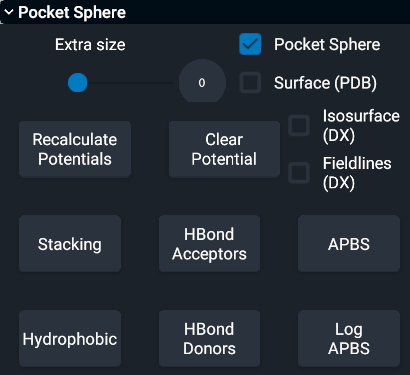
\includegraphics[width=0.5\textwidth]{figures/methods/umol_ps-main.png}
      \caption{\label{fig:methods/umol_ps-main} Main instance of the PSMenu. It gives access to the core functionalities of the visualization pipeline.}
    \end{figure}

    The size of the PS can be increased by means of the \textit{Extra size} slider, which also updates the pocket/non-pocket selections. The translucid sphere that represents the PS can be toggled on or off with the \textit{Pocket Sphere} toggle, while the cartoon-licorice based representations can be changed to surface representations with the \textit{Surface (PDB)} toggle.

    The potential fields can be calculated by clicking the \textit{Recalculate Potentials} button, although this will not display any potential by its own. THe potential field of interest can be displayed individually by clicking on its respective button, be it \textit{Stacking}, \textit{HBond Acceptors}, \textit{APBS}, \textit{Hydrophobic}, \textit{HBond Donors} or \textit{Log APBS}. The displayed potentials can be cleared from the screen by clicking on the \textit{Clear Potential} button.

    The user can switch between the two volumetric representations available for the potential fields by toggling on or off the \textit{Isosurface (DX)} toggle. The \textit{Fieldlines (DX)} toggle is not described in this work, as it is in an experimental stage and it just seeks to simplify the usage of a third volumetric representation already provided by UnityMol (i.e. fieldlines).

  \subsection{Potentials Calculation}
    Whenever the \textit{Recalculate Potentials} from figure \ref{fig:methods/umol_ps-main} button is pressed, information about the PS (such as center, diameter, path to the PDB file and whether the system corresponds to RNA) is stored into a JSON file. A Python script is then executed to proceed with the calculation pipeline. The algorithm recovers the center and diameter of the sphere from the JSON file to approximate the binding pocket of the system as a cube in the same position. This volume is then separated into small subunits of volume, regularly spaced in any given axis (although the amount of subunits may change between axes). The subunits are further discretized into points of a three-dimensional NumPy matrix.

    The matrix is filled with values for the different potentials, by employing the models described before. Atom selections are handled by MDA, while the actual numerical operations use NumPy methods to increase performance. In the case of APBS potentials, the APBS pipeline must be followed beforehand until obtaining the DX file with the results. These are then taken by the Python scripts to perform further adjustments and operations.

    Once the potential grids are populated with values, points that correspond to positions outside the actual PS observed in UnityMol are set to $0$, as they are outside the region of interest. Furthermore, grid points whose position are in close proximity to pocket atoms are also set to 0, as they are placed in a volume already occupied by said atoms and are not plausible positions for a pharmacophore. This process is referred to here as \textbf{trimming}. The distance treshold for proximity is set to {3 \AA} for trimming.

    Finally, each potential grid is stored twice, both as a JSON file and as a DX file. This is not only a measure to communicate the results between Python and UnityMol, but also allows for a fast display of the different grids by just loading the precomputed data files instead of performing the potential calculations every time.

  \subsection{Potentials Visualization}
    A first idea for how to repersent three-dimensional grids of data in an intuitive way was to generate \textit{clouds} of points, which would ideally be denser in regions where the values for the potentials are higher. This appropriately named \textbf{cloud representation} of volumetric data was implemented from scratch in UnityMol.

    The precomputed JSON files are loaded by a C\# script that populates a three-dimensional array with the potential values. It then takes advantage of optimized multiprocessing routines to build the vertices and triangles of a cubic mesh, giving to each vertex a color that corresponds to its respective potential value. These meshes are then handled by a shader GPU program that assigns semi-transparent colors to the triangles according to their neighbouring vertices: more saturated and opaque colors imply higher potential values. Note that grid points whose potential values are equal to 0 are still represented by vertices and triangles in the mesh, but the shader colors them totally transparent.

    Alternatively, the potential grids can be visualized using an \textbf{isosurface representation}. In this case, the PSMenu only takes care of using the internal UnityMol APIs to open the DX file of interest and building the representation. For the potentials that require negative values (namely \textit{APBS}, \textit{LogAPBS} and \textit{Hydrophobicity}), two isosurface representations are built: one for the positive values and another for the negative ones. This allows to color them appropriately and further differentiate them by using distinct configurations of \textit{opaque}, \textit{translucid} or \textit{wireframe} between the two.


%%%%%%%%%%%%%%%%%%%%%%%%%%%%%%%%%%%%%%%%%%%%%%%%%%%%%%%%%%%%%%%%%%%%%%%%%%%%%%%%
\section{Benchmarking}
  A collection of 10 protein based (table \ref{tab:methods/benchmark_prot}) and 10 RNA based (table \ref{tab:methods/benchmark_rna}) PDB files was assembled to carry out benchmarks on the potential calculations and their visualization. The protein structures were chosen from a literature review of binding pockets with different characteristics of interest. The RNA structures were obtained as a representative set of complexes from the RNA-ligand interaction database Hariboss \cite{hariboss_2022}.

  \begin{table}[H]
    \caption{\label{tab:methods/benchmark_prot} [TODO: description].}
    \centering
    \begin{tabular}{ccccp{1.5in}p{1.5in}c}
      \hline
      PDB  & Ligands & Atoms & pKD   & Description                                & Comments                                                                   & Source                            \\ \hline
      1BG0 & ADP     & 2817  & -     & arginine kinase                            & negatively charged pocket - NO3 and Mg also participate in the active site & \cite{benchmark_negative_2000}    \\ \hline
      1EBY & BEB     & 1522  & 9.70  & HIV-1 protease in complex with inhibitor   & strong pocket affinity                                                     & \cite{benchmark_strong_2021}      \\ \hline
      1EHE & HEM     & 3100  & -     & cytochrome P450NOR                         & positively charged pocket                                                  & \cite{benchmark_positive_2001}    \\ \hline
      1H7L & TYD     & 1976  & -     & glycosyltransferase                        & -                                                                          & \cite{benchmark_1h7l_2001}        \\ \hline
      1IQJ & XMH     & 2241  & -     & serine protease - blood coagulation factor & -                                                                          & to be published                   \\ \hline
      1OFZ & FUL-FUC & 4891  & 4.62  & fungal lectin                              & hydrogen bonds                                                             & \cite{hbonds_2023}                \\ \hline
      3DD0 & EZL     & 2074  & 9.00  & carbonic anhydrase II                      & strong pocket affinity                                                     & \cite{benchmark_strong_2021}      \\ \hline
      3EE4 & MYR     & 2320  & -     & Mn/Fe oxidase from M. tuberculosis         & hydrophobic pocket                                                         & \cite{benchmark_hydrophobic_2009} \\ \hline
      5M9W & 7GR     & 4856  & 2.24  & thermolysin in complex with inhibitor      & hydrophobic pocket                                                         & \cite{hydrophobic_2017}           \\ \hline
      6E9A & J0S     & 1705  & 11.92 & HIV-1 protease                             & strongest pocket affinity reported in PDBbind                              & \cite{pdbbind_2004}               \\ \hline
    \end{tabular}
  \end{table}

  \begin{table}[H]
    \caption{\label{tab:methods/benchmark_rna} [TODO: description]. All structures are taken from Hariboss \cite{hariboss_2022}.}
    \centering
    \begin{tabular}{ccccp{1.5in}p{1.5in}}
      \hline
      PDB  & Ligands & Atoms & pKD  & Description                                                 & Comments                                                \\ \hline
      1AKX & ARG     & 965   & -    & HIV-2 trans activating region RNA complex with argininamide & confusing for APBS pipeline - takes ligand as a protein \\ \hline
      1I9V & NMY     & 1632  & 3.47 & phenylalanine transfer RNA                                  & -                                                       \\ \hline
      2ESJ & LIV     & 900   & -    & 16S-rRNA A site                                             & -                                                       \\ \hline
      4F8U & SIS     & 922   & -    & ribosomal decoding site                                     & -                                                       \\ \hline
      5KX9 & 6YG     & 2323  & -    & FMN riboswitch                                              & -                                                       \\ \hline
      6TF3 & 3AT     & 1112  & -    & NAD+ riboswitch                                             & -                                                       \\ \hline
      7OAX & SPM     & 4404  & -    & RNA aptamer                                                 & large RNA                                               \\ \hline
      7OAX & V5Z     & 4404  & -    & RNA aptamer                                                 & large RNA                                               \\ \hline
      5BJO & 747     & 1568  & -    & corn RNA aptamer in complex with DFHO                       & large SiteScore (1.090) on Hariboss                     \\ \hline
      8EYV & 747     & 1954  & -    & beetroot dimer bound to DFHO                                & largest DScore (1.187) on Hariboss                      \\ \hline
    \end{tabular}
  \end{table}

%%%%%%%%%%%%%%%%%%%%%%%%%%%%%%%%%%%%%%%%%%%%%%%%%%%%%%%%%%%%%%%%%%%%%%%%%%%%%%%%

  %%% describe all the experiments performed and their statistical analysis
\chapter{Results} % at least 10, maximum 40 pages

%%%%%%%%%%%%%%%%%%%%%%%%%%%%%%%%%%%%%%%%%%%%%%%%%%%%%%%%%%%%%%%%%%%%%%%%%%%%%%%%
\section{Characterization of Physicochemical Properties}
  \subsection{Stacking Potential}
    \paragraph*{Obtaining the Datasets}\mbox{}\\
      A total of $83500$ protein structure files were downloaded from the PDB, some of which also contained ligands. Similarly, $3032$ structures with protein and nucleic acid complexes where downloaded, with the presence of ligands in some of them. From these two datasets, $22786$ unique ligand IDs were observed. The CIF files for these ligands were also downloaded from the PDB.

    \paragraph*{Detecting Aromatic Groups in Ligands}\mbox{}\\
      The first method of detection (parsing the SMILES strings) found aromaticity in $18211$ ligands from the dataset, while the second method (simple topological examination of the structures) found aromatic groups in $19096$ ligand files. From these ligands, $388$ were detected only by the first method, while $1273$ were detected only by the second method, meaning that the detection methods disagreed in the case of $1661$ ligands (figure \ref{fig:results/stacking}).

      \begin{figure}[H]
        \centering
        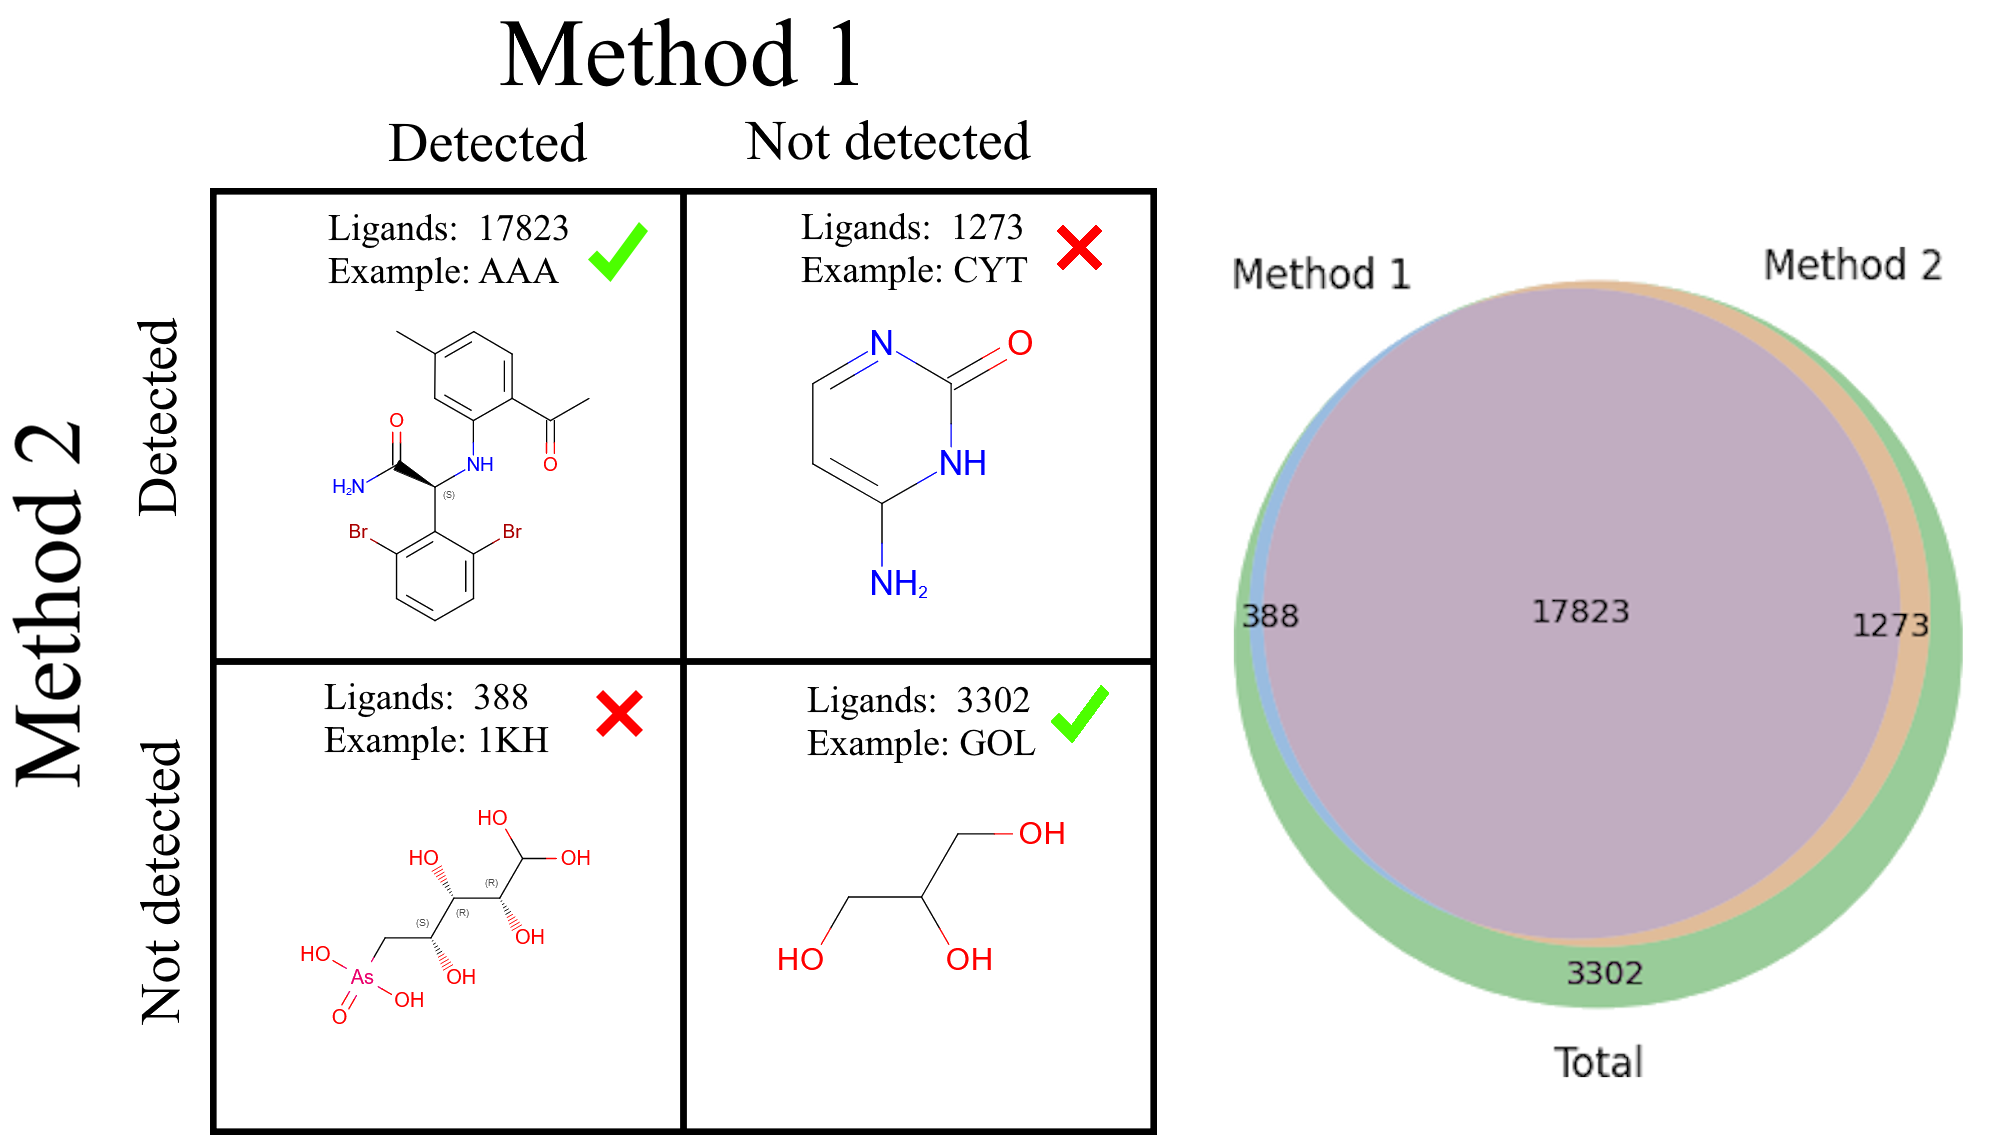
\includegraphics[width=0.8\textwidth]{figures/results/stacking.png}
        \caption{\label{fig:results/stacking} [TODO: description]}
      \end{figure}

      Some CIF files from the dataset had faulty SMILES strings (such as including the ligand name as a placeholder) or did not report correctly the aromaticity of the ligands. An example of the latter is the nucleic acid cytosine (CYT in figure \ref{fig:results/stacking}), which is not properly identified as aromatic despite being a classic example of a very biologically relevant aromatic group. This also was observed in uracyl and other pyrimidines.

      % 18211 method 1
      % 18404 method 2 --> should be more
      % 1273  detected only by method 2
      % 388   detected only by method 1

      The opposite situation also happened, where the SMILES string apparently contained aromatic atoms because lowercase symbols were found. However, this sometimes corresponded unrelated heavy atoms. An example of this occurance is the ligand 1KH in figure \ref{fig:results/stacking}, whose arsenic atom is represented by "As" in the SMILES string, so the first method recognized the lowercase "s" as an aromatic sulfur. The second method however immediatly discarded the ligand as it is acyclic.

      Some other instances with complex combinations of aromatic and non-aromatic rings (oftentimes connected by one or two atoms) presented problems for the second method, while being correctly reported in the first method (figure [TODO: add some examples in appendix\_ii]). For these reasons, these $1661$ were manually inspected to clarify whether aromaticity was present or not. At the end of this process, $18298$ ligands (accounting for $80.3 \% $ of the original dataset) were found to present a combined total of $34807$ aromatic groups (on average, 1.9 aromatic groups per ligand).

    \paragraph*{Sampling of Aromatic Interactions}\mbox{}\\
      a

      [TODO: statistical results from the dataset]

    \paragraph*{Model Definition}\mbox{}\\
      a

      [TODO: description of how the model shape was defined as a gaussian based in the histograms of distance and alpha angles, as well as its parameters mu and sigma]

      [TODO: show the donuts formed by the multivariate gaussian model]

  \subsection{Hydrogen Bonds Potential}
    [TODO: show the spheres formed by the univariate gaussian model]

    [TODO: description of the simultaneous positions where the ligand can have an ideal angle for the given distance]

  \subsection{Electrostatic Potential}
    [TODO: show the christmas tree effect and compare it to logAPBS]

    [TODO: show the log and trimmed log plots]


%%%%%%%%%%%%%%%%%%%%%%%%%%%%%%%%%%%%%%%%%%%%%%%%%%%%%%%%%%%%%%%%%%%%%%%%%%%%%%%%
\section{Development of Visualization Methods}
  \subsection{Graphical User Interface}
    % Pocket Sphere stuff
    [TODO: pocket sphere and changing its size vs pocket sphere off]

    [TODO: cartoon vs surface representation]

    [TODO: trimmed vs not trimmed sphere]

  \subsection{Potentials Visualization}
    % Representation of the potential grids in UnityMol
    [TODO: cloud vs isosurface]


%%%%%%%%%%%%%%%%%%%%%%%%%%%%%%%%%%%%%%%%%%%%%%%%%%%%%%%%%%%%%%%%%%%%%%%%%%%%%%%%
\section{Benchmarking}
  \subsection{Protein Systems}
    [TODO]

  \subsection{RNA Systems}
    [TODO]


%%%%%%%%%%%%%%%%%%%%%%%%%%%%%%%%%%%%%%%%%%%%%%%%%%%%%%%%%%%%%%%%%%%%%%%%%%%%%%%%

  %%% critical analysis of the results obtained and frames them in the context of the international literature
\chapter{Discussion} % at least 5, maximum 10 pages

[TEMPLATE: critical analysis of the results obtained and frames them in the context of the international literature.]

  %%% briefly summarize the key outcome of the project and outlines any future directions
\chapter{Conclusions and future perspectives} % at least 1 page, not more than 2 pages

[TODO: implement hydrophobicity in RNA]

[TODO: implement calculations directly within Unity]


  \cleardoublepage \pagenumbering{gobble} % stop page number after last numbered chapter
  \bibliographystyle{ieeetr}
\bibliography{biblio}

  \chapter*{Appendix I}
\addcontentsline{toc}{chapter}{Appendix I}  

[TEMPLATE: Used if more pages of materials and methods are required. Not included in 85 pages count.]
  %%% used for replication data or other materials that do not fit the results section. Not included in 85 pages count.
\chapter*{Appendix II}
\addcontentsline{toc}{chapter}{Appendix II}

%%%%%%%%%%%%%%%%%%%%%%%%%%%%%%%%%%%%%%%%%%%%%%%%%%%%%%%%%%%%%%%%%%%%%%%%%%%%%%%% STACKING POTENTIAL
\begin{figure}[H]
  \centering
  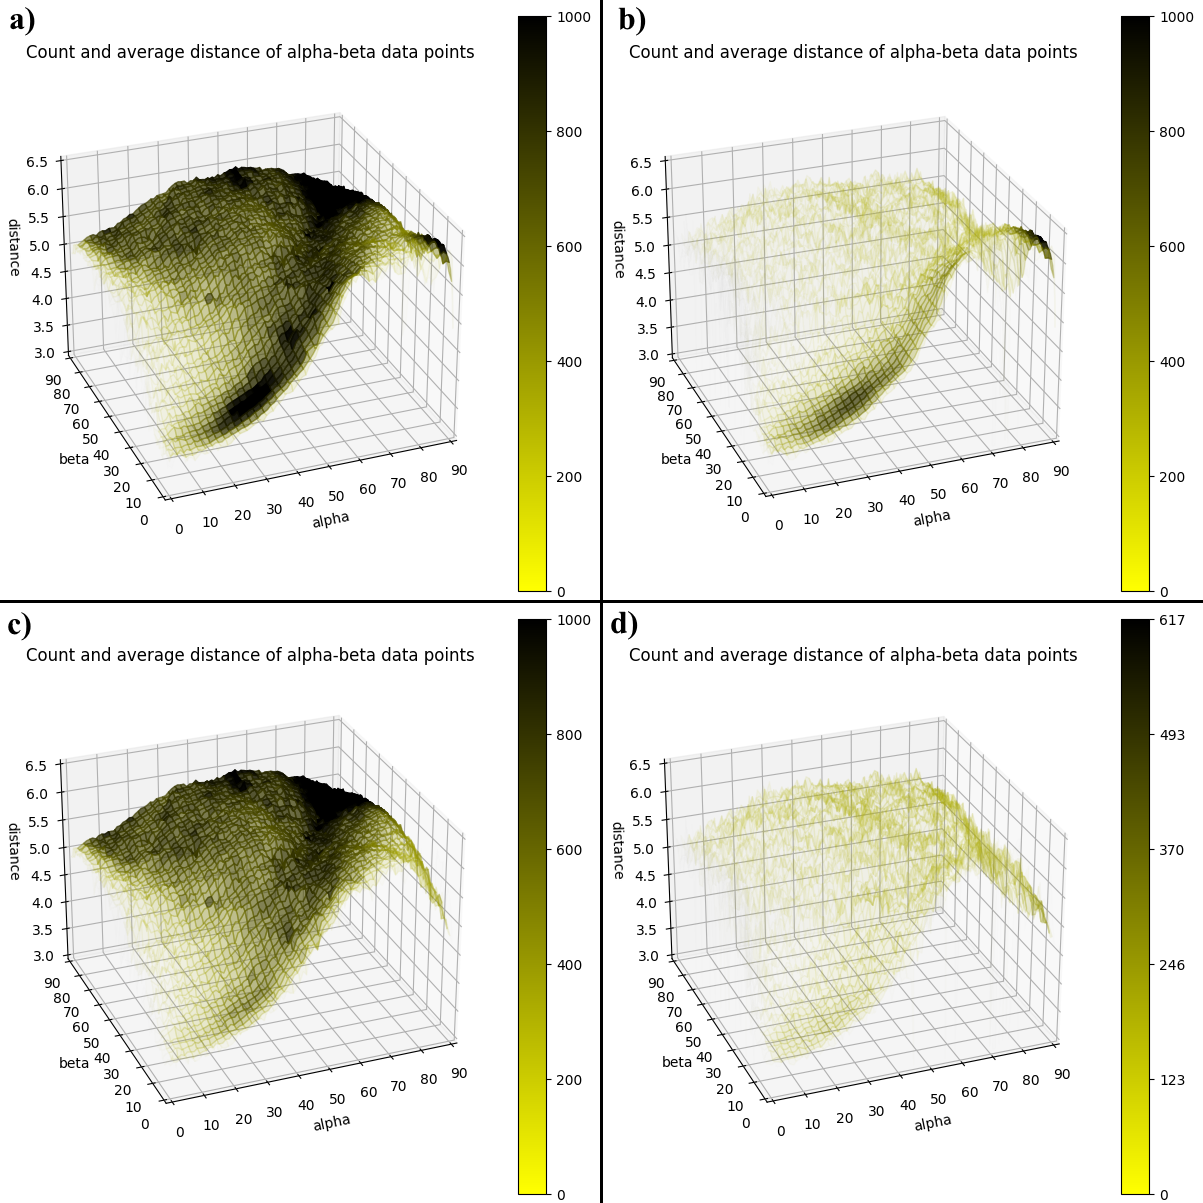
\includegraphics[width=0.7\textwidth]{figures/appendix/stacking_sampling.png}
  \caption{\label{fig:appendix/stacking_sampling} [TODO: description]}
\end{figure}

%%%%%%%%%%%%%%%%%%%%%%%%%%%%%%%%%%%%%%%%%%%%%%%%%%%%%%%%%%%%%%%%%%%%%%%%%%%%%%%% BENCHMARK PROTEIN

%%%%%%%%%%%%%%%%%%%%%%%%%%%%%%%%%%%%%%%%%%%%%%%%%%%%%%%%%%%%%%%%%%%%%%%%%%%%%%%% BENCHMARK RNA

%%%%%%%%%%%%%%%%%%%%%%%%%%%%%%%%%%%%%%%%%%%%%%%%%%%%%%%%%%%%%%%%%%%%%%%%%%%%%%%%


\end{document}

%%%%%%%%%%%%%%%%%%%%%%%%%%%%%%%%%%%%%%%%%%%%%%%%%%%%%%%%%%%%%%%%%%%%%%%%%%%%%%%% TEMPLATES
% \begin{figure}[H]
%   \centering
%   \includegraphics[width=1\textwidth]{figures/name}
%   \caption{\label{fig:name} Description. }
% \end{figure}
